%!TEX options = -shell-escape
\documentclass[a4paper]{article}

\usepackage{amsmath, amssymb}
\usepackage{listings}
\usepackage{courier}
\usepackage{color}
\usepackage{pgfplots}
\usepackage{subcaption}
\usepackage{fontspec}
\usepackage{minted}
\setmonofont{DejaVu Sans Mono}

\pgfplotsset{compat=newest}
\usetikzlibrary{plotmarks}
\usetikzlibrary{arrows.meta}
\usepgfplotslibrary{patchplots}

\definecolor{light-gray}{gray}{0.7}

\newcommand{\norm}[1]{\left\lVert#1\right\rVert}
\DeclareMathOperator{\diag}{diag}

\author{H.T. Stoppels (University of Groningen)}
\title{{\sc nbalss} homework 4}

% \lstdefinestyle{myCustomMatlabStyle}{
%   language=Julia,
%   tabsize=4,
%   showspaces=false,
%   showstringspaces=false
% }

% \lstset{basicstyle=\footnotesize\ttfamily,breaklines=true,style=myCustomMatlabStyle}
% \lstset{frame=tblr,rulecolor=\color{light-gray}}

\begin{document}
  \maketitle 

  We consider again the familiar equation. We consider again the familiar equation.We consider again the familiar equation.We consider again the familiar equation.We consider again the familiar equation.We consider again the familiar equation.

  \paragraph{a} In Figure~\ref{fig:solutions} we see three non-trivial solutions at $\mu = 200,$ together with their norms as $\mu$ gets larger.


  \begin{figure}[h]
    \begin{subfigure}[b]{0.5\textwidth}
      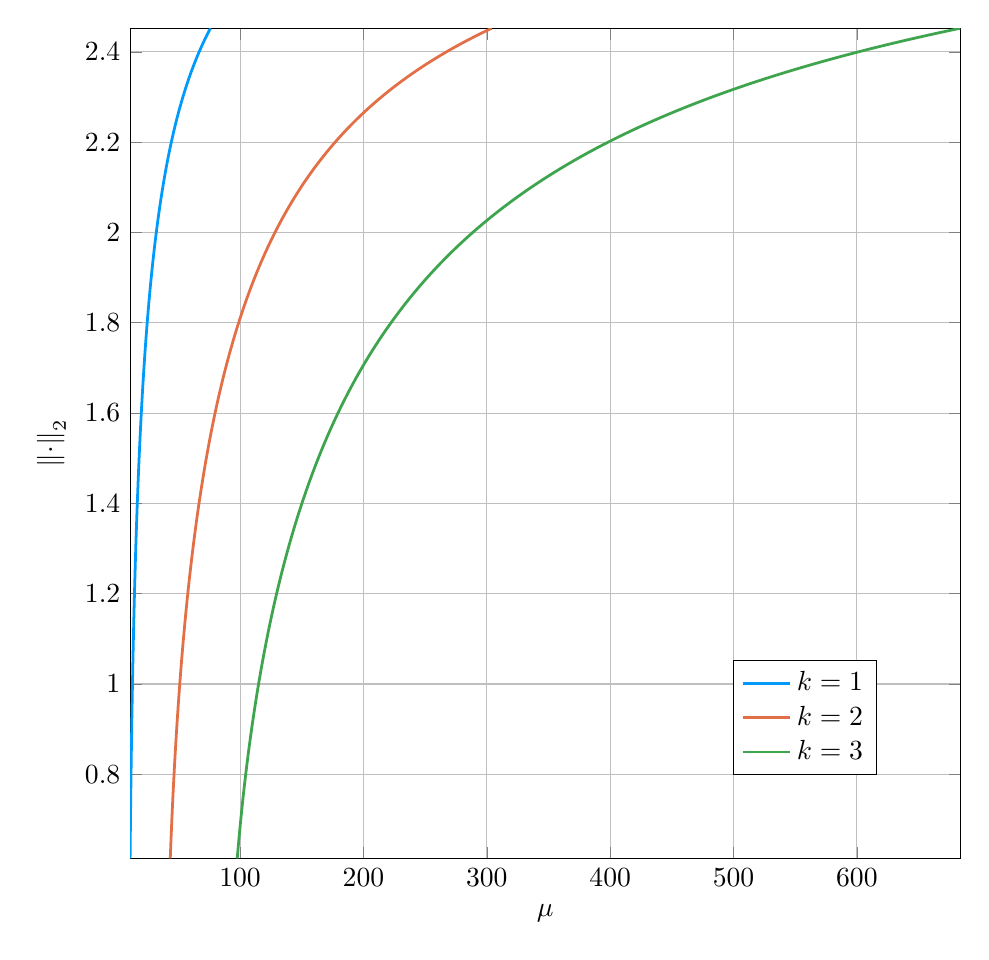
\begin{tikzpicture}
\begin{axis}[width = {\linewidth}, ymax = {2.452237324104191}, height = {\linewidth},
    legend style={at={(0.9,0.1)},anchor=south east}, xlabel = {$\mu$}, {unbounded coords=jump,     xshift = 0.0mm,
    yshift = 0.0mm,
    axis background/.style={fill={rgb,1:red,1.00000000;green,1.00000000;blue,1.00000000}}
, grid = major}, ylabel = {$\norm{\cdot}_2$}, ymin = {0.6137482854178079}, xmax = {683.838279520865}, xmin = {10.85634382949168}]\addplot+ [color = {rgb,1:red,0.00000000;green,0.60560316;blue,0.97868012},
draw opacity=1.0,
line width=1,
solid,mark = none,
mark size = 2.0,
mark options = {
    color = {rgb,1:red,0.00000000;green,0.00000000;blue,0.00000000}, draw opacity = 1.0,
    fill = {rgb,1:red,0.00000000;green,0.60560316;blue,0.97868012}, fill opacity = 1.0,
    line width = 1,
    rotate = 0,
    solid
}]coordinates {
(10.85634382949168, 0.6137482854178079)
(11.019597120160729, 0.6594309077605753)
(11.182850410829777, 0.7013815376663717)
(11.346103701498825, 0.740257961397065)
(11.509356992167872, 0.7765429938301521)
(11.672610282836922, 0.8106038879975136)
(11.835863573505968, 0.8427280085233041)
(11.999116864175015, 0.8731454369055732)
(12.162370154844066, 0.9020439313689711)
(12.325623445513111, 0.929579187891071)
(12.488876736182158, 0.9558820929925184)
(12.652130026851209, 0.9810639831564152)
(12.815383317520254, 1.0052205438902742)
(12.978636608189303, 1.0284347564590814)
(13.14188989885835, 1.0507791629099046)
(13.305143189527401, 1.0723176334195699)
(13.468396480196446, 1.0931067639127485)
(13.631649770865494, 1.1131969946756504)
(13.794903061534544, 1.1326335154433393)
(13.95815635220359, 1.1514570049768926)
(14.121409642872637, 1.1697042408538278)
(14.284662933541687, 1.1874086064018743)
(14.447916224210733, 1.2046005153232406)
(14.611169514879782, 1.2213077698607586)
(14.774422805548829, 1.2375558648602076)
(14.937676096217876, 1.2533682474484398)
(15.100929386886925, 1.268766540041585)
(15.264182677555972, 1.2837707328558776)
(15.427435968225021, 1.2983993508974592)
(15.590689258894068, 1.3126695994720858)
(15.753942549563115, 1.326597491517446)
(15.917195840232164, 1.3401979594747153)
(16.08044913090121, 1.353484953946774)
(16.24370242157026, 1.3664715310127662)
(16.40695571223931, 1.3791699297625233)
(16.570209002908356, 1.3915916413648246)
(16.733462293577404, 1.4037474707788327)
(16.89671558424645, 1.415647592049586)
(17.059968874915498, 1.4273015979886907)
(17.22322216558455, 1.4387185449253974)
(17.386475456253596, 1.4499069931159063)
(17.549728746922643, 1.4608750433175208)
(17.71298203759169, 1.4716303699653306)
(17.876235328260737, 1.4821802513311704)
(18.039488618929788, 1.4925315969951474)
(18.202741909598835, 1.5026909729178983)
(18.365995200267882, 1.5126646243658883)
(18.52924849093693, 1.5224584969110153)
(18.692501781605976, 1.5320782556993477)
(18.855755072275027, 1.5415293031607125)
(19.019008362944074, 1.5508167953111567)
(19.18226165361312, 1.5599456567828098)
(19.34551494428217, 1.5689205947009903)
(19.508768234951216, 1.5777461115147207)
(19.672021525620266, 1.586426516876099)
(19.835274816289314, 1.5949659386531638)
(19.99852810695836, 1.6033683331524935)
(20.161781397627408, 1.6116374946198428)
(20.325034688296455, 1.6197770640801625)
(20.488287978965506, 1.627790537572395)
(20.651541269634553, 1.6356812738288515)
(20.8147945603036, 1.6434525014444172)
(20.978047850972647, 1.6511073255761826)
(21.141301141641694, 1.6586487342107719)
(21.304554432310745, 1.6660796040327195)
(21.467807722979792, 1.6734027059246672)
(21.63106101364884, 1.6806207101270016)
(21.794314304317886, 1.6877361910824213)
(21.957567594986934, 1.6947516319885663)
(22.120820885655984, 1.7016694290798335)
(22.28407417632503, 1.7084918956578201)
(22.44732746699408, 1.7152212658880686)
(22.610580757663126, 1.7218596983794727)
(22.773834048332173, 1.7284092795612946)
(22.937087339001224, 1.7348720268715287)
(23.10034062967027, 1.7412498917692714)
(23.263593920339318, 1.7475447625828346)
(23.426847211008365, 1.7537584672043345)
(23.590100501677412, 1.7598927756406084)
(23.753353792346463, 1.7659494024298836)
(23.91660708301551, 1.7719300089324266)
(24.079860373684557, 1.777836205503268)
(24.243113664353604, 1.783669553554165)
(24.40636695502265, 1.7894315675116867)
(24.569620245691702, 1.7951237166775915)
(24.73287353636075, 1.8007474269974577)
(24.896126827029796, 1.806304082742889)
(25.059380117698844, 1.8117950281125028)
(25.22263340836789, 1.8172215687562472)
(25.38588669903694, 1.8225849732275845)
(25.54913998970599, 1.8278864743675405)
(25.712393280375036, 1.8331272706245085)
(25.875646571044083, 1.8383085273134145)
(26.03889986171313, 1.843431377817433)
(26.20215315238218, 1.848496924735622)
(26.365406443051228, 1.8535062409791898)
(26.528659733720275, 1.8584603708192546)
(26.691913024389322, 1.8633603308886761)
(26.85516631505837, 1.868207111140294)
(27.01841960572742, 1.8730016757639476)
(27.181672896396467, 1.8777449640642803)
(27.344926187065514, 1.882437891301484)
(27.50817947773456, 1.8870813494966963)
(27.67143276840361, 1.8916762082039837)
(27.83468605907266, 1.8962233152504284)
(27.997939349741706, 1.9007234974460132)
(28.161192640410754, 1.905177561264725)
(28.3244459310798, 1.9095862934982322)
(28.487699221748848, 1.9139504618835872)
(28.6509525124179, 1.9182708157060298)
(28.814205803086946, 1.92254808637817)
(28.977459093755993, 1.9267829879966774)
(29.14071238442504, 1.930976217877417)
(29.303965675094094, 1.9351284570701353)
(29.467218965763138, 1.939240370853579)
(29.630472256432185, 1.9433126092119282)
(29.793725547101232, 1.9473458072934375)
(29.95697883777028, 1.9513405858520008)
(30.120232128439326, 1.9552975516724946)
(30.28348541910838, 1.959217297980521)
(30.446738709777424, 1.9631004048372835)
(30.60999200044647, 1.9669474395202595)
(30.77324529111552, 1.9707589568901969)
(30.936498581784566, 1.9745354997451308)
(31.099751872453616, 1.978277599161885)
(31.263005163122667, 1.981985774825622)
(31.42625845379171, 1.9856605353479146)
(31.589511744460758, 1.989302378573874)
(31.752765035129805, 1.9929117918787176)
(31.916018325798856, 1.9964892524542432)
(32.0792716164679, 2.0000352275856232)
(32.242524907136946, 2.0035501749188898)
(32.405778197806, 2.007034542719492)
(32.56903148847505, 2.010488770122304)
(32.732284779144095, 2.0139132873733825)
(32.89553806981314, 2.0173085160638147)
(33.05879136048219, 2.0206748693559864)
(33.22204465115123, 2.0240127522025304)
(33.38529794182028, 2.027322561558244)
(33.54855123248933, 2.030604686585285)
(33.71180452315838, 2.033859508851819)
(33.875057813827425, 2.0370874025244574)
(34.03831110449648, 2.0402887345546685)
(34.20156439516552, 2.0434638648593686)
(34.36481768583457, 2.046613146495968)
(34.52807097650362, 2.049736925832018)
(34.69132426717267, 2.0528355427097105)
(34.854577557841715, 2.055909330605337)
(35.01783084851076, 2.058958616784006)
(35.18108413917981, 2.0619837224496633)
(35.344337429848856, 2.0649849628906867)
(35.5075907205179, 2.067962647621139)
(35.67084401118696, 2.0709170805178863)
(35.834097301856005, 2.073848559953671)
(35.99735059252505, 2.076757378926347)
(36.16060388319409, 2.079643825184356)
(36.323857173863146, 2.0825081813485893)
(36.48711046453219, 2.0853507250307612)
(36.65036375520124, 2.0881717289484554)
(36.81361704587029, 2.090971461036835)
(36.976870336539335, 2.093750184557299)
(37.14012362720838, 2.0965081582030507)
(37.303376917877436, 2.099245636201702)
(37.46663020854648, 2.1019628684151197)
(37.62988349921553, 2.104660100436436)
(37.79313678988458, 2.1073375736844664)
(37.956390080553625, 2.1099955254955196)
(38.119643371222665, 2.112634189212742)
(38.28289666189172, 2.1152537942730354)
(38.446149952560766, 2.117854566291658)
(38.60940324322981, 2.120436727144586)
(38.77265653389886, 2.1230004950486463)
(38.935909824567915, 2.125546084639576)
(39.099163115236955, 2.1280737070480096)
(39.26241640590601, 2.1305835699734983)
(39.425669696575056, 2.1330758777566)
(39.5889229872441, 2.135550831449086)
(39.75217627791315, 2.1380086288823694)
(39.9154295685822, 2.140449464734181)
(40.078682859251245, 2.1428735305935205)
(40.24193614992029, 2.1452810150239863)
(40.40518944058934, 2.1476721036255064)
(40.56844273125839, 2.1500469790945034)
(40.73169602192744, 2.152405821282574)
(40.89494931259649, 2.1547488072537138)
(41.05820260326553, 2.1570761113401002)
(41.22145589393458, 2.159387905196531)
(41.384709184603636, 2.1616843578535154)
(41.547962475272676, 2.1639656357690726)
(41.71121576594172, 2.1662319028792827)
(41.87446905661077, 2.168483320647589)
(42.03772234727982, 2.170720048112957)
(42.20097563794887, 2.1729422419368434)
(42.36422892861792, 2.1751500564490676)
(42.527482219286966, 2.1773436436925895)
(42.690735509956006, 2.179523153467222)
(42.85398880062506, 2.1816887333723445)
(43.0172420912941, 2.1838405288485827)
(43.180495381963155, 2.1859786832185333)
(43.34374867263221, 2.188103337726554)
(43.50700196330125, 2.190214631577622)
(43.670255253970296, 2.192312701975302)
(43.83350854463935, 2.194397684158863)
(43.99676183530839, 2.1964697114394998)
(44.160015125977445, 2.1985289152358165)
(44.3232684166465, 2.2005754251084264)
(44.48652170731554, 2.202609368793829)
(44.64977499798459, 2.204630872237488)
(44.81302828865363, 2.206640059626225)
(44.97628157932268, 2.2086370534198303)
(45.13953486999173, 2.2106219743820326)
(45.30278816066078, 2.2125949416107558)
(45.46604145132983, 2.2145560725677114)
(45.62929474199887, 2.216505483107371)
(45.79254803266792, 2.218443287505278)
(45.95580132333696, 2.22036959848578)
(46.11905461400602, 2.2222845272491174)
(46.28230790467506, 2.2241881834979855)
(46.44556119534411, 2.2260806754634954)
(46.60881448601316, 2.2279621099305813)
(46.772067776682206, 2.2298325922628903)
(46.93532106735126, 2.23169222642712)
(47.09857435802031, 2.2335411150168762)
(47.261827648689355, 2.235379359275997)
(47.4250809393584, 2.2372070591214226)
(47.58833423002744, 2.239024313165562)
(47.751587520696496, 2.2408312187382173)
(47.914840811365536, 2.242627871908047)
(48.07809410203459, 2.2444143675035906)
(48.24134739270364, 2.246190799133857)
(48.404600683372685, 2.24795725920852)
(48.56785397404173, 2.249713838957652)
(48.731107264710786, 2.25146062845112)
(48.89436055537983, 2.2531977166175454)
(49.05761384604888, 2.2549251912629122)
(49.220867136717935, 2.256643139088772)
(49.384120427386975, 2.2583516457101336)
(49.547373718056015, 2.2600507956729405)
(49.71062700872507, 2.2617406724712557)
(49.873880299394116, 2.263421358564082)
(50.03713359006316, 2.26509293539184)
(50.20038688073221, 2.266755483392562)
(50.363640171401265, 2.268409082017741)
(50.526893462070305, 2.270053809747871)
(50.69014675273936, 2.2716897441077144)
(50.85340004340841, 2.2733169616812408)
(51.01665333407745, 2.274935538126316)
(51.17990662474651, 2.276545548189069)
(51.34315991541555, 2.278147065718024)
(51.506413206084595, 2.2797401636779395)
(51.66966649675364, 2.2813249141633998)
(51.83291978742269, 2.28290138841214)
(51.99617307809174, 2.2844696568181297)
(52.15942636876078, 2.2860297889443983)
(52.32267965942984, 2.28758185353565)
(52.48593295009888, 2.2891259185306048)
(52.64918624076793, 2.2906620510741527)
(52.812439531436986, 2.2921903175292377)
(52.975692822106026, 2.293710783488585)
(53.13894611277508, 2.2952235137861354)
(53.30219940344412, 2.296728572508344)
(53.46545269411317, 2.298226023005232)
(53.62870598478221, 2.299715927901255)
(53.79195927545126, 2.301198349105953)
(53.955212566120316, 2.3026733478244426)
(54.118465856789356, 2.3041409845676926)
(54.28171914745841, 2.305601319162629)
(54.44497243812745, 2.307054410762065)
(54.608225728796505, 2.3085003178544268)
(54.77147901946556, 2.3099390982733485)
(54.9347323101346, 2.3113708092070695)
(55.09798560080365, 2.3127955072076665)
(55.2612388914727, 2.3142132482001476)
(55.42449218214174, 2.315624087491352)
(55.58774547281079, 2.317028079778727)
(55.750998763479835, 2.3184252791589377)
(55.91425205414889, 2.3198157391363248)
(56.07750534481793, 2.3211995126312286)
(56.24075863548698, 2.3225766519881543)
(56.40401192615603, 2.3239472089838187)
(56.56726521682508, 2.3253112348350333)
(56.73051850749413, 2.3266687802064765)
(56.89377179816318, 2.328019895218323)
(57.057025088832226, 2.3293646294537376)
(57.22027837950127, 2.3307030319662667)
(57.38353167017031, 2.3320351512870743)
(57.54678496083936, 2.333361035432081)
(57.71003825150841, 2.3346807319089717)
(57.87329154217746, 2.335994287724091)
(58.03654483284651, 2.337301749389224)
(58.199798123515556, 2.3386031629282615)
(58.3630514141846, 2.339898573883766)
(58.52630470485366, 2.341188027323407)
(58.689557995522705, 2.3424715678463213)
(58.85281128619175, 2.343749239589345)
(59.016064576860806, 2.345021086233155)
(59.179317867529846, 2.346287151008308)
(59.342571158198886, 2.347547476701185)
(59.50582444886793, 2.3488021056598294)
(59.66907773953699, 2.3500510797997114)
(59.832331030206035, 2.3512944406093754)
(59.99558432087508, 2.3525322291560187)
(60.158837611544136, 2.3537644860909643)
(60.322090902213176, 2.3549912516550577)
(60.48534419288223, 2.356212565683976)
(60.648597483551285, 2.3574284676134454)
(60.811850774220325, 2.3586389964843915)
(60.97510406488938, 2.359844190947996)
(61.13835735555842, 2.3610440892706777)
(61.301610646227466, 2.36223872933899)
(61.464863936896506, 2.3634281486644624)
(61.62811722756556, 2.3646123843883418)
(61.791370518234615, 2.3657914732862735)
(61.954623808903655, 2.366965451772912)
(62.11787709957271, 2.3681343559064465)
(62.28113039024175, 2.3692982213930813)
(62.4443836809108, 2.3704570835914245)
(62.60763697157986, 2.371610977516813)
(62.7708902622489, 2.3727599378455912)
(62.93414355291795, 2.3739039989193023)
(63.09739684358699, 2.3750431947488235)
(63.26065013425604, 2.376177559018443)
(63.42390342492508, 2.377307125089872)
(63.58715671559413, 2.378431926006201)
(63.75041000626319, 2.379551994495783)
(63.91366329693223, 2.3806673629760797)
(64.07691658760129, 2.3817780635574324)
(64.24016987827032, 2.382884128046788)
(64.40342316893938, 2.3839855879513623)
(64.56667645960842, 2.385082474482252)
(64.72992975027748, 2.3861748185580103)
(64.89318304094652, 2.3872626508081245)
(65.05643633161557, 2.3883460015765)
(65.21968962228462, 2.3894249009248507)
(65.38294291295365, 2.390499378636058)
(65.54619620362271, 2.391569464217485)
(65.70944949429176, 2.392635186904224)
(65.87270278496081, 2.3936965756623176)
(66.03595607562985, 2.394753659191922)
(66.1992093662989, 2.3958064659304266)
(66.36246265696795, 2.3968550240555375)
(66.525715947637, 2.397899361488294)
(66.68896923830604, 2.398939505896072)
(66.8522225289751, 2.3999754846955264)
(67.01547581964414, 2.4010073250554886)
(67.17872911031318, 2.4020350538998394)
(67.34198240098223, 2.403058697910328)
(67.50523569165128, 2.4040782835293544)
(67.66848898232034, 2.4050938369627177)
(67.83174227298937, 2.406105384182314)
(67.99499556365843, 2.407112950928814)
(68.15824885432747, 2.4081165627142895)
(68.32150214499653, 2.4091162448248076)
(68.48475543566558, 2.4101120223229913)
(68.64800872633462, 2.411103920050539)
(68.81126201700367, 2.4120919626307176)
(68.97451530767272, 2.413076174470816)
(69.13776859834176, 2.4140565797645617)
(69.3010218890108, 2.41503320249451)
(69.46427517967986, 2.4160060664344067)
(69.6275284703489, 2.4169751951514993)
(69.79078176101795, 2.417940612008834)
(69.954035051687, 2.4189023401675174)
(70.11728834235605, 2.419860402588948)
(70.2805416330251, 2.420814822037003)
(70.44379492369414, 2.4217656210802327)
(70.6070482143632, 2.4227128220939753)
(70.77030150503225, 2.4236564472624926)
(70.9335547957013, 2.4245965185810334)
(71.09680808637033, 2.425533057857908)
(71.26006137703938, 2.4264660867165113)
(71.42331466770842, 2.427395626597318)
(71.58656795837749, 2.4283216987598704)
(71.74982124904653, 2.4292443242847224)
(71.91307453971558, 2.430163524075363)
(72.07632783038463, 2.431079318860121)
(72.23958112105367, 2.431991729194032)
(72.40283441172272, 2.432900775460697)
(72.56608770239177, 2.4338064778740987)
(72.72934099306082, 2.434708856480411)
(72.89259428372986, 2.4356079311597765)
(73.05584757439891, 2.4365037216280587)
(73.21910086506796, 2.437396247438583)
(73.382354155737, 2.438285527983835)
(73.54560744640605, 2.4391715824971625)
(73.7088607370751, 2.4400544300544356)
(73.87211402774416, 2.4409340895756944)
(74.0353673184132, 2.441810579826776)
(74.19862060908225, 2.442683919420915)
(74.36187389975129, 2.4435541268203314)
(74.52512719042035, 2.4444212203377935)
(74.6883804810894, 2.44528521813816)
(74.85163377175844, 2.4461461382399055)
(75.01488706242749, 2.447003998516633)
(75.17814035309652, 2.4478588166985533)
(75.34139364376558, 2.448710610373951)
(75.50464693443462, 2.44955939699064)
(75.66790022510368, 2.4504051938574016)
(75.83115351577273, 2.451248018145382)
(75.99440680644177, 2.4520878868895006)
};
\addlegendentry{$k = 1$}
\addplot+ [color = {rgb,1:red,0.88887350;green,0.43564919;blue,0.27812294},
draw opacity=1.0,
line width=1,
solid,mark = none,
mark size = 2.0,
mark options = {
    color = {rgb,1:red,0.00000000;green,0.00000000;blue,0.00000000}, draw opacity = 1.0,
    fill = {rgb,1:red,0.88887350;green,0.43564919;blue,0.27812294}, fill opacity = 1.0,
    line width = 1,
    rotate = 0,
    solid
}]coordinates {
(43.422723263872186, 0.6137489530035443)
(44.07569654603568, 0.6594317368403398)
(44.728669828199166, 0.7013825365100819)
(45.38164311036266, 0.7402591371714722)
(46.03461639252615, 0.776544352787178)
(46.68758967468964, 0.8106054356168284)
(47.340562956853134, 0.842729749623926)
(47.99353623901663, 0.8731473757350743)
(48.646509521180114, 0.9020460716761819)
(49.29948280334361, 0.9295815329863694)
(49.9524560855071, 0.9558846457984018)
(50.605429367670595, 0.9810667462504941)
(51.25840264983409, 1.0052235195419936)
(51.911375931997576, 1.0284379466615723)
(52.56434921416107, 1.0507825694076305)
(53.21732249632456, 1.072321257732525)
(53.87029577848805, 1.0931106073578012)
(54.52326906065154, 1.1132010583854282)
(55.17624234281503, 1.132637800382992)
(55.829215624978524, 1.1514615119590603)
(56.48218890714202, 1.1697089705520483)
(57.135162189305504, 1.1874135593626196)
(57.788135471469005, 1.2046056919767734)
(58.44110875363249, 1.2213131705309468)
(59.094082035795985, 1.237561489773393)
(59.74705531795948, 1.2533740967415077)
(60.400028600122965, 1.268772613769313)
(61.05300188228645, 1.2837770309976009)
(61.70597516444995, 1.2984058733632016)
(62.35894844661345, 1.312676346108136)
(63.01192172877693, 1.3266044621114754)
(63.66489501094043, 1.3402051537604867)
(64.31786829310391, 1.3534923716084457)
(64.9708415752674, 1.3664791716888691)
(65.6238148574309, 1.3791777930496227)
(66.27678813959439, 1.391599726820886)
(66.92976142175789, 1.4037557779263357)
(67.58273470392137, 1.4156561203783955)
(68.23570798608486, 1.42731034695873)
(68.88868126824835, 1.4387275139690958)
(69.54165455041185, 1.4499161816404917)
(70.19462783257534, 1.460884450707122)
(70.84760111473884, 1.4716399955829365)
(71.50057439690232, 1.4821900945204736)
(72.15354767906581, 1.4925416570822052)
(72.80652096122931, 1.5027012492127227)
(73.4594942433928, 1.5126751161639016)
(74.1124675255563, 1.5224692034944018)
(74.76544080771978, 1.5320891763383275)
(75.41841408988327, 1.5415404371147208)
(76.07138737204676, 1.5508281418299206)
(76.72436065421024, 1.5599572151074184)
(77.37733393637374, 1.5689323640647779)
(78.03030721853725, 1.5777580911442033)
(78.68328050070073, 1.5864387059917961)
(79.33625378286422, 1.5949783364703578)
(79.98922706502772, 1.6033809388819604)
(80.6422003471912, 1.6116503074685151)
(81.29517362935471, 1.619790083251756)
(81.9481469115182, 1.6278037622679955)
(82.60112019368168, 1.6356947032474793)
(83.25409347584517, 1.6434661347834951)
(83.90706675800865, 1.6511211620320507)
(84.56004004017217, 1.658662772979105)
(85.21301332233564, 1.6660938443089626)
(85.86598660449914, 1.6734171469043955)
(86.51895988666263, 1.6806353510062886)
(87.17193316882611, 1.6877510310581831)
(87.8249064509896, 1.6947666702588648)
(88.4778797331531, 1.7016846648441732)
(89.1308530153166, 1.7085073281174092)
(89.78382629748008, 1.715236894246071)
(90.43679957964358, 1.7218755218412596)
(91.08977286180706, 1.7284252973346392)
(91.74274614397055, 1.7348882381668118)
(92.39571942613406, 1.741266295799689)
(93.04869270829755, 1.747561358564554)
(93.70166599046104, 1.753775254356644)
(94.35463927262452, 1.7599097531861043)
(95.00761255478801, 1.7659665695945639)
(95.66058583695151, 1.771947364945847)
(96.313559119115, 1.7778537495986442)
(96.9665324012785, 1.7836872849684997)
(97.61950568344199, 1.7894494854858392)
(98.27247896560547, 1.7951418204563914)
(98.92545224776896, 1.8007657158297732)
(99.57842552993246, 1.8063225558817175)
(100.23139881209595, 1.8118136848150255)
(100.88437209425945, 1.8172404082838973)
(101.53734537642293, 1.8226039948461021)
(102.19031865858642, 1.8279056773470173)
(102.84329194074992, 1.8331466542394537)
(103.49626522291342, 1.838328090842761)
(104.1492385050769, 1.8434511205446082)
(104.8022117872404, 1.8485168459485473)
(105.45518506940388, 1.853526339970321)
(106.10815835156737, 1.8584806468856112)
(106.76113163373087, 1.863380783331845)
(107.41410491589436, 1.8682277392664584)
(108.06707819805786, 1.873022478883883)
(108.72005148022133, 1.8777659414933867)
(109.37302476238483, 1.8824590423597676)
(110.02599804454833, 1.8871026735087943)
(110.67897132671182, 1.8916977044991417)
(111.3319446088753, 1.8962449831625188)
(111.9849178910388, 1.9007453363135272)
(112.63789117320229, 1.9051995704307503)
(113.29086445536578, 1.909608472310476)
(113.94383773752928, 1.913972809694339)
(114.59681101969277, 1.9182933318721551)
(115.24978430185625, 1.922570770261115)
(115.90275758401974, 1.9268058389624316)
(116.55573086618324, 1.9309992352965117)
(117.20870414834674, 1.9351516403176194)
(117.86167743051024, 1.9392637193090019)
(118.51465071267371, 1.9433361222593246)
(119.16762399483721, 1.9473694843212976)
(119.8205972770007, 1.9513644262532648)
(120.47357055916419, 1.9553215548445104)
(121.12654384132769, 1.9592414633250321)
(121.77951712349117, 1.9631247317604081)
(122.43249040565468, 1.9669719274324513)
(123.08546368781815, 1.9707836052062397)
(123.73843696998165, 1.9745603078840963)
(124.39141025214515, 1.9783025665471132)
(125.04438353430864, 1.9820109008846851)
(125.69735681647212, 1.9856858195126037)
(126.35033009863561, 1.9893278202801603)
(127.00330338079911, 1.9929373905667322)
(127.65627666296258, 1.9965150075682405)
(128.30924994512608, 2.0000611385739546)
(128.96222322728957, 2.0035762412339713)
(129.61519650945306, 2.007060763817782)
(130.26816979161654, 2.0105151454642676)
(130.92114307378006, 2.01393981642346)
(131.57411635594354, 2.017335198290402)
(132.22708963810703, 2.0207017042313913)
(132.88006292027052, 2.024039739202948)
(133.533036202434, 2.027349700163732)
(134.18600948459752, 2.0306319762797154)
(134.838982766761, 2.0338869491228695)
(135.4919560489245, 2.037114992863571)
(136.14492933108798, 2.0403164744570126)
(136.79790261325147, 2.043491753823822)
(137.45087589541495, 2.0466411840250798)
(138.10384917757847, 2.0497651114319844)
(138.75682245974195, 2.0528638758903277)
(139.40979574190544, 2.055937810879992)
(140.06276902406893, 2.058987243669633)
(140.7157423062324, 2.0620124954667194)
(141.36871558839593, 2.065013881563115)
(142.02168887055942, 2.0679917114763473)
(142.6746621527229, 2.0709462890867063)
(143.3276354348864, 2.07387791277034)
(143.98060871704988, 2.0767868755284726)
(144.63358199921336, 2.079673465112882)
(145.28655528137688, 2.0825379641477704)
(145.93952856354036, 2.085380650248143)
(146.59250184570385, 2.0882017961348214)
(147.24547512786734, 2.091001669746209)
(147.89844841003082, 2.0937805343468905)
(148.55142169219434, 2.096538648633231)
(149.20439497435783, 2.0992762668359917)
(149.8573682565213, 2.10199363882014)
(150.5103415386848, 2.1046910101818934)
(151.16331482084829, 2.1073686223431234)
(151.81628810301177, 2.110026712643162)
(152.4692613851753, 2.1126655144281523)
(153.12223466733877, 2.1152852571379674)
(153.77520794950226, 2.1178861663908193)
(154.42818123166575, 2.120468464065589)
(155.08115451382923, 2.1230323683819985)
(155.73412779599272, 2.1255780939786484)
(156.38710107815623, 2.1281058519890164)
(157.04007436031972, 2.1306158501154626)
(157.6930476424832, 2.1331082927013276)
(158.3460209246467, 2.135583380801147)
(158.99899420681018, 2.13804131224907)
(159.6519674889737, 2.140482281725534)
(160.30494077113718, 2.142906480822227)
(160.95791405330067, 2.1453140981054086)
(161.61088733546416, 2.147705319177636)
(162.26386061762764, 2.15008032673795)
(162.91683389979116, 2.1524393006405376)
(163.56980718195464, 2.1547824179519512)
(164.22278046411813, 2.157109853006911)
(164.87575374628162, 2.1594217774627325)
(165.5287270284451, 2.161718360352417)
(166.1817003106086, 2.163999768136458)
(166.8346735927721, 2.166266164753376)
(167.4876468749356, 2.168517711669047)
(168.14062015709908, 2.1707545679248357)
(168.79359343926257, 2.1729768901845814)
(169.44656672142605, 2.1751848327804586)
(170.09954000358954, 2.1773785477577667)
(170.75251328575305, 2.1795581849186396)
(171.4054865679165, 2.181723891864744)
(172.05845985008003, 2.1838758140389807)
(172.7114331322435, 2.1860140947662003)
(173.364406414407, 2.1881388752929913)
(174.01737969657052, 2.190250294826543)
(174.67035297873397, 2.1923484905726123)
(175.3233262608975, 2.1944335977726306)
(175.97629954306095, 2.1965057497399587)
(176.62927282522446, 2.1985650778953234)
(177.28224610738792, 2.200611711801451)
(177.93521938955143, 2.202645779196931)
(178.58819267171495, 2.2046674060293077)
(179.2411659538784, 2.20667671648745)
(179.89413923604192, 2.208673833033192)
(180.5471125182054, 2.2106588764322757)
(181.2000858003689, 2.212631965784622)
(181.8530590825324, 2.2145932185539303)
(182.5060323646959, 2.2165427505966306)
(183.15900564685938, 2.2184806761902163)
(183.81197892902287, 2.2204071080609533)
(184.46495221118636, 2.222322157411002)
(185.11792549334982, 2.224225933944951)
(185.77089877551333, 2.226118545895783)
(186.4238720576768, 2.2280001000502945)
(187.0768453398403, 2.2298707017739727)
(187.72981862200382, 2.231730455035346)
(188.38279190416728, 2.233579462429826)
(189.0357651863308, 2.2354178252030494)
(189.6887384684943, 2.237245643273728)
(190.3417117506578, 2.2390630152560376)
(190.9946850328213, 2.2408700384815226)
(191.6476583149848, 2.242666809020576)
(192.30063159714828, 2.2444534217034495)
(192.95360487931177, 2.2462299701408575)
(193.60657816147526, 2.2479965467441496)
(194.25955144363874, 2.2497532427450775)
(194.91252472580223, 2.2515001482151598)
(195.56549800796574, 2.253237352084662)
(196.21847129012923, 2.2549649421611875)
(196.87144457229272, 2.2566830051479094)
(197.5244178544562, 2.258391626661426)
(198.1773911366197, 2.260090891249272)
(198.83036441878318, 2.261780882407078)
(199.4833377009467, 2.2634616825954)
(200.13631098311018, 2.2651333732562082)
(200.78928426527366, 2.2667960348290617)
(201.44225754743715, 2.268449746766968)
(202.09523082960064, 2.270094587551928)
(202.74820411176415, 2.2717306347101895)
(203.4011773939276, 2.2733579648272078)
(204.05415067609113, 2.2749766535623044)
(204.70712395825458, 2.276586775663065)
(205.3600972404181, 2.2781884049794536)
(206.01307052258161, 2.2797816144776575)
(206.66604380474507, 2.2813664762536727)
(207.3190170869086, 2.28294306154664)
(207.97199036907205, 2.284511440751917)
(208.62496365123556, 2.2860716834339168)
(209.27793693339902, 2.287623858338708)
(209.93091021556253, 2.28916803340637)
(210.58388349772605, 2.2907042757831317)
(211.2368567798895, 2.292232651833281)
(211.88983006205302, 2.2937532271508503)
(212.54280334421648, 2.295266066571102)
(213.19577662638, 2.2967712341817905)
(213.84874990854345, 2.2982687933342247)
(214.50172319070697, 2.2997588066541357)
(215.15469647287048, 2.3012413360523345)
(215.80766975503394, 2.302716442735193)
(216.46064303719746, 2.3041841872149282)
(217.11361631936091, 2.3056446293197026)
(217.76658960152443, 2.3070978282035504)
(218.4195628836879, 2.30854384235612)
(219.0725361658514, 2.3099827296122526)
(219.72550944801492, 2.311414547161378)
(220.37848273017838, 2.312839351556764)
(221.0314560123419, 2.3142571987245906)
(221.68442929450535, 2.315668143972867)
(222.33740257666886, 2.3170722420001986)
(222.99037585883235, 2.318469546904396)
(223.64334914099584, 2.319860112190941)
(224.29632242315935, 2.3212439907813)
(224.9492957053228, 2.3226212350211046)
(225.60226898748633, 2.3239918966881765)
(226.25524226964978, 2.325356027000434)
(226.9082155518133, 2.3267136766236467)
(227.5611888339768, 2.3280648956790726)
(228.21416211614027, 2.3294097337509574)
(228.86713539830376, 2.330748239893911)
(229.52010868046725, 2.332080462640158)
(230.17308196263076, 2.333406450006668)
(230.82605524479425, 2.3347262495021694)
(231.47902852695773, 2.336039908134041)
(232.13200180912125, 2.337347472415092)
(232.78497509128476, 2.338648988370235)
(233.43794837344825, 2.339944501543036)
(234.09092165561174, 2.3412340570021715)
(234.74389493777525, 2.34251769934777)
(235.3968682199387, 2.343795472717655)
(236.04984150210223, 2.3450674207934803)
(236.70281478426568, 2.3463335868067743)
(237.3557880664292, 2.3475940135448803)
(238.00876134859269, 2.3488487433568004)
(238.66173463075617, 2.3500978181589507)
(239.3147079129197, 2.351341279440819)
(239.96768119508314, 2.352579168270533)
(240.62065447724666, 2.353811525300345)
(241.27362775941012, 2.3550383907720196)
(241.92660104157363, 2.356259804522146)
(242.5795743237371, 2.357475805987358)
(243.2325476059006, 2.35868643420948)
(243.88552088806412, 2.359891727840583)
(244.53849417022758, 2.3610917251479706)
(245.1914674523911, 2.362286464019078)
(245.84444073455455, 2.363475981966305)
(246.49741401671807, 2.3646603161317636)
(247.15038729888153, 2.365839503291959)
(247.80336058104504, 2.3670135798623955)
(248.45633386320856, 2.368182581902113)
(249.10930714537201, 2.3693465451181517)
(249.76228042753553, 2.3705055048699517)
(250.415253709699, 2.371659496173682)
(251.0682269918625, 2.3728085537065056)
(251.721200274026, 2.3739527118107793)
(252.37417355618948, 2.375092004498191)
(253.027146838353, 2.376226465453832)
(253.68012012051645, 2.3773561280402125)
(254.33309340267996, 2.378481025301211)
(254.98606668484342, 2.3796011899659684)
(255.63903996700694, 2.380716654452725)
(256.2920132491704, 2.381827450872597)
(256.94498653133394, 2.3829336110332986)
(257.5979598134974, 2.384035166442809)
(258.2509330956609, 2.3851321483129877)
(258.9039063778244, 2.38622458756313)
(259.5568796599879, 2.3873125148234777)
(260.2098529421514, 2.388395960438673)
(260.86282622431486, 2.389474954471168)
(261.51579950647834, 2.390549526704576)
(262.1687727886419, 2.391619706646982)
(262.8217460708053, 2.392685523534201)
(263.47471935296886, 2.39374700633299)
(264.1276926351323, 2.394804183744216)
(264.78066591729583, 2.3958570842059745)
(265.43363919945926, 2.3969057358966683)
(266.0866124816228, 2.3979501667380347)
(266.7395857637863, 2.3989904043981407)
(267.3925590459498, 2.4000264762943235)
(268.04553232811327, 2.4010584095960974)
(268.69850561027675, 2.4020862312280205)
(269.35147889244024, 2.40310996787251)
(270.0044521746037, 2.4041296459726365)
(270.6574254567672, 2.405145291734856)
(271.31039873893076, 2.4061569311317266)
(271.9633720210942, 2.4071645899045704)
(272.61634530325773, 2.4081682935661073)
(273.2693185854212, 2.409168067403049)
(273.9222918675847, 2.4101639364786562)
(274.5752651497482, 2.411155925635266)
(275.2282384319117, 2.4121440594967742)
(275.8812117140752, 2.4131283624710953)
(276.5341849962387, 2.41410885875258)
(277.1871582784022, 2.4150855723244042)
(277.8401315605657, 2.416058526960924)
(278.49310484272917, 2.4170277462299983)
(279.14607812489265, 2.41799325349528)
(279.79905140705614, 2.418955071918477)
(280.4520246892196, 2.419913224461582)
(281.1049979713831, 2.4208677338890734)
(281.7579712535466, 2.4218186227700835)
(282.4109445357101, 2.422765913480542)
(283.06391781787363, 2.4237096282052875)
(283.71689110003706, 2.4246497889401515)
(284.3698643822006, 2.4255864174940176)
(285.02283766436403, 2.4265195354908484)
(285.6758109465276, 2.4274491643716885)
(286.32878422869106, 2.4283753253966425)
(286.98175751085455, 2.4292980396468224)
(287.63473079301804, 2.4302173280262753)
(288.2877040751815, 2.4311332112638793)
(288.940677357345, 2.4320457099152217)
(289.5936506395085, 2.4329548443644446)
(290.246623921672, 2.4338606348260754)
(290.8995972038355, 2.4347631013468254)
(291.55257048599896, 2.435662263807371)
(292.2055437681625, 2.436558141924108)
(292.85851705032593, 2.437450755250886)
(293.5114903324895, 2.438340123180719)
(294.1644636146529, 2.4392262649474747)
(294.81743689681645, 2.4401091996275404)
(295.47041017897993, 2.4409889461414713)
(296.1233834611434, 2.441865523255614)
(296.7763567433069, 2.4427389495837133)
(297.4293300254704, 2.4436092435884924)
(298.0823033076339, 2.4444764235832204)
(298.73527658979737, 2.4453405077332553)
(299.38824987196085, 2.446201514057569)
(300.0412231541244, 2.447059460430255)
(300.6941964362878, 2.4479143645820103)
(301.34716971845137, 2.4487662441016096)
(302.0001430006148, 2.4496151164373514)
(302.65311628277834, 2.450460998898492)
(303.3060895649418, 2.451303908656656)
(303.9590628471053, 2.4521438627472394)
};
\addlegendentry{$k = 2$}
\addplot+ [color = {rgb,1:red,0.24222430;green,0.64327509;blue,0.30444865},
draw opacity=1.0,
line width=1,
solid,mark = none,
mark size = 2.0,
mark options = {
    color = {rgb,1:red,0.00000000;green,0.00000000;blue,0.00000000}, draw opacity = 1.0,
    fill = {rgb,1:red,0.24222430;green,0.64327509;blue,0.30444865}, fill opacity = 1.0,
    line width = 1,
    rotate = 0,
    solid
}]coordinates {
(97.69118278869499, 0.6137500667207719)
(99.16022313138214, 0.6594331199722109)
(100.62926347406928, 0.7013842028523297)
(102.09830381675643, 0.7402610986795248)
(103.56734415944356, 0.7765466198901909)
(105.03638450213069, 0.8106080174558162)
(106.50542484481784, 0.8427326542377271)
(107.97446518750499, 0.8731506102092285)
(109.44350553019214, 0.902049642264264)
(110.91254587287926, 0.9295854452105572)
(112.38158621556641, 0.9558889045338789)
(113.85062655825357, 0.9810713557970548)
(115.3196669009407, 1.005228483685466)
(116.78870724362785, 1.028443268726837)
(118.257747586315, 1.0507882523047716)
(119.72678792900213, 1.072327303997233)
(121.19582827168927, 1.0931170191869644)
(122.66486861437642, 1.1132078376686123)
(124.13390895706357, 1.1326449487304204)
(125.60294929975069, 1.1514690307265916)
(127.07198964243784, 1.1697168608635207)
(128.541029985125, 1.1874218221299602)
(130.01007032781212, 1.2046143279180876)
(131.47911067049927, 1.2213221801868848)
(132.94815101318642, 1.2375708735219617)
(134.41719135587357, 1.2533838548115235)
(135.8862316985607, 1.2687827462526426)
(137.35527204124782, 1.2837875378603214)
(138.82431238393497, 1.2984167544557825)
(140.29335272662212, 1.3126876011747632)
(141.76239306930927, 1.326616090798599)
(143.23143341199642, 1.340217155624642)
(144.70047375468357, 1.353504746123463)
(146.1695140973707, 1.366491918252494)
(147.63855444005785, 1.3791909109896157)
(149.107594782745, 1.3916132154006446)
(150.57663512543212, 1.403769636350094)
(152.04567546811924, 1.4156703477960118)
(153.5147158108064, 1.4273249424701309)
(154.98375615349354, 1.4387424766283752)
(156.4527964961807, 1.4499315104597168)
(157.92183683886785, 1.4609001446598577)
(159.390877181555, 1.4716560536075183)
(160.85991752424212, 1.4822065155230397)
(162.32895786692927, 1.4925584399395182)
(163.79799820961642, 1.5027183927747898)
(165.26703855230355, 1.5126926192564003)
(166.7360788949907, 1.522487064920969)
(168.20511923767785, 1.5321073948826416)
(169.67415958036497, 1.5415590115424844)
(171.14319992305212, 1.550847070890688)
(172.61224026573925, 1.5599764975362855)
(174.08128060842643, 1.5689519985839755)
(175.55032095111355, 1.577778076464597)
(177.01936129380073, 1.586459040814236)
(178.48840163648785, 1.5949990194869825)
(179.95744197917497, 1.603401968777399)
(181.42648232186212, 1.611671682920995)
(182.89552266454925, 1.619811802934166)
(184.36456300723643, 1.627825824848848)
(185.83360334992355, 1.6357171073918135)
(187.3026436926107, 1.6434888791537423)
(188.77168403529785, 1.6511442452888165)
(190.24072437798498, 1.658686193781907)
(191.7097647206721, 1.6661176013169197)
(193.17880506335928, 1.6734412387768731)
(194.6478454060464, 1.680659776403496)
(196.11688574873355, 1.68777578864173)
(197.5859260914207, 1.6947917586922776)
(199.05496643410785, 1.7017100827933898)
(200.52400677679498, 1.7085330742512177)
(201.9930471194821, 1.7152629672365391)
(203.46208746216928, 1.721901920364116)
(204.9311278048564, 1.7284520200696432)
(206.40016814754355, 1.7349152837980872)
(207.8692084902307, 1.7412936630160305)
(209.33824883291783, 1.7475890460597272)
(210.80728917560498, 1.7538032608296463)
(212.27632951829213, 1.7599380773414137)
(213.74536986097922, 1.7659952101423713)
(215.2144102036664, 1.771976320602265)
(216.68345054635358, 1.7778830190859047)
(218.1524908890407, 1.7837168670151253)
(219.62153123172783, 1.7894793788268197)
(221.09057157441498, 1.795172023833327)
(222.5596119171021, 1.8007962279910077)
(224.02865225978928, 1.8063533755824766)
(225.4976926024764, 1.8118448108175218)
(226.96673294516353, 1.8172718393574367)
(228.4357732878507, 1.8226357297671694)
(229.90481363053783, 1.827937714899374)
(231.37385397322495, 1.8331789932142013)
(232.8428943159121, 1.8383607300384104)
(234.31193465859926, 1.8434840587671364)
(235.78097500128644, 1.8485500820114555)
(237.25001534397353, 1.8535598726946698)
(238.7190556866607, 1.8585144751000593)
(240.18809602934783, 1.8634149058726848)
(241.657136372035, 1.8682621549776384)
(243.12617671472213, 1.873057186617028)
(244.59521705740923, 1.8778009401078084)
(246.06425740009644, 1.8824943307224848)
(247.53329774278356, 1.8871382504945284)
(249.00233808547068, 1.891733568990321)
(250.47137842815783, 1.896281134049279)
(251.94041877084496, 1.9007817724936982)
(253.40945911353208, 1.9052362908098535)
(254.87849945621926, 1.9096454758017072)
(256.3475397989064, 1.9140100952185493)
(257.81658014159353, 1.9183308983578404)
(259.2856204842807, 1.9226086166443832)
(260.75466082696784, 1.9268439641869888)
(262.22370116965493, 1.9310376383136272)
(263.69274151234214, 1.9351903200861027)
(265.16178185502923, 1.939302674795168)
(266.63082219771644, 1.9433753524369632)
(268.09986254040354, 1.9474089881716388)
(269.5689028830907, 1.951404202764939)
(271.03794322577784, 1.9553616030135195)
(272.506983568465, 1.9592817821547006)
(273.9760239111521, 1.9631653202613486)
(275.4450642538393, 1.9670127846225234)
(276.91410459652644, 1.9708247301105)
(278.38314493921354, 1.9746016995347675)
(279.8521852819007, 1.9783442239835272)
(281.32122562458784, 1.9820528231532446)
(282.79026596727493, 1.9857280056667326)
(284.25930630996214, 1.9893702693802626)
(285.72834665264924, 1.9929801016801347)
(287.1973869953364, 1.9965579797691537)
(288.66642733802354, 2.0001043709434185)
(290.1354676807107, 2.0036197328598107)
(291.60450802339784, 2.0071045137945545)
(293.073548366085, 2.0105591528932116)
(294.54258870877214, 2.0139840804124503)
(296.01162905145924, 2.0173797179538915)
(297.4806693941464, 2.020746478690371)
(298.94970973683354, 2.0240847675848856)
(300.4187500795207, 2.0273949816025256)
(301.88779042220784, 2.0306775099156478)
(303.356830764895, 2.0339327341025446)
(304.8258711075821, 2.0371610283398716)
(306.2949114502693, 2.0403627595890512)
(307.7639517929564, 2.0435382877768817)
(309.23299213564354, 2.046687965970568)
(310.7020324783307, 2.04981214054738)
(312.1710728210178, 2.0529111513591327)
(313.640113163705, 2.0559853318916796)
(315.1091535063921, 2.059035009419593)
(316.57819384907924, 2.062060505156211)
(318.0472341917664, 2.06506213439922)
(319.51627453445354, 2.0680402066719115)
(320.9853148771407, 2.070995025860295)
(322.45435521982785, 2.073926890346188)
(323.923395562515, 2.0768360931364316)
(325.3924359052021, 2.0797229219883757)
(326.8614762478893, 2.0825876595317405)
(328.3305165905764, 2.0854305833870033)
(329.79955693326355, 2.0882519662804095)
(331.2685972759507, 2.0910520761557327)
(332.7376376186378, 2.093831176282891)
(334.20667796132494, 2.096589525363522)
(335.67571830401215, 2.0993273776336205)
(337.14475864669924, 2.1020449829633376)
(338.6137989893864, 2.1047425869540297)
(340.08283933207355, 2.1074204310326543)
(341.55187967476064, 2.1100787525435925)
(343.0209200174478, 2.112717784837985)
(344.489960360135, 2.1153377573606575)
(345.95900070282215, 2.1179388957347296)
(347.42804104550925, 2.120521421843947)
(348.8970813881964, 2.1230855539128504)
(350.36612173088355, 2.1256315065848153)
(351.83516207357064, 2.1281594909980477)
(353.30420241625785, 2.130669714859599)
(354.773242758945, 2.1331623825174515)
(356.24228310163215, 2.1356376950307427)
(357.71132344431925, 2.1380958502381855)
(359.1803637870064, 2.1405370428247306)
(360.64940412969355, 2.142961464386543)
(362.11844447238065, 2.1453693034943164)
(363.5874848150678, 2.147760745755007)
(365.056525157755, 2.1501359738720036)
(366.52556550044216, 2.152495167703808)
(367.99460584312925, 2.1548385043212464)
(369.4636461858164, 2.1571661580632737)
(370.93268652850355, 2.1594783005914)
(372.40172687119065, 2.1617751009427835)
(373.87076721387785, 2.164056725582035)
(375.339807556565, 2.1663233384517575)
(376.8088478992521, 2.168575101021867)
(378.27788824193925, 2.1708121723377345)
(379.7469285846264, 2.173034709067167)
(381.2159689273135, 2.1752428655462728)
(382.68500927000065, 2.177436793824245)
(384.15404961268786, 2.179616643707078)
(385.623089955375, 2.181782562800265)
(387.0921302980621, 2.183934696550492)
(388.56117064074925, 2.1860731882863678)
(390.0302109834364, 2.188198179258199)
(391.4992513261235, 2.1903098086768606)
(392.9682916688107, 2.1924082137517624)
(394.43733201149786, 2.194493529727955)
(395.906372354185, 2.196565889922383)
(397.3754126968721, 2.1986254257593267)
(398.84445303955926, 2.2006722668050345)
(400.3134933822464, 2.2027065408015822)
(401.7825337249336, 2.204728373699971)
(403.2515740676207, 2.2067378896924956)
(404.72061441030786, 2.208735211244381)
(406.189654752995, 2.210720459124736)
(407.6586950956821, 2.2126937524368113)
(409.12773543836926, 2.214655208647609)
(410.59677578105646, 2.2166049436168325)
(412.06581612374356, 2.218543071625216)
(413.5348564664307, 2.2204697054022415)
(415.00389680911786, 2.222384956153251)
(416.47293715180496, 2.2242889335859903)
(417.94197749449205, 2.226181745936569)
(419.41101783717926, 2.2280634999948825)
(420.88005817986635, 2.2299343011294908)
(422.3490985225535, 2.231794253311964)
(423.81813886524066, 2.233643459140731)
(425.28717920792775, 2.2354820198644187)
(426.7562195506149, 2.237310035404702)
(428.2252598933021, 2.239127604378692)
(429.69430023598926, 2.240934824120846)
(431.16334057867635, 2.2427317907044375)
(432.6323809213635, 2.24451859896258)
(434.10142126405066, 2.246295342508821)
(435.57046160673787, 2.2480621137573182)
(437.03950194942496, 2.2498190039426067)
(438.5085422921121, 2.2515661031389658)
(439.97758263479926, 2.2533035002793933)
(441.44662297748636, 2.255031283174205)
(442.9156633201735, 2.2567495385292613)
(444.3847036628607, 2.258458351963823)
(445.85374400554787, 2.260157808028065)
(447.32278434823496, 2.261847990220236)
(448.7918246909221, 2.263528981003486)
(450.26086503360926, 2.2652008618223562)
(451.72990537629636, 2.2668637131189557)
(453.19894571898357, 2.268517614348818)
(454.6679860616707, 2.270162643996451)
(456.1370264043578, 2.271798879590586)
(457.60606674704496, 2.2734263977191396)
(459.0751070897321, 2.2750452740438756)
(460.5441474324192, 2.2766555833147994)
(462.0131877751064, 2.2782573993842736)
(463.48222811779357, 2.279850795220865)
(464.9512684604807, 2.281435842922928)
(466.4203088031678, 2.283012613731941)
(467.88934914585496, 2.2845811780455803)
(469.3583894885421, 2.286141605430559)
(470.8274298312293, 2.287693964635224)
(472.2964701739164, 2.289238323601914)
(473.76551051660357, 2.2907747494791)
(475.2345508592906, 2.29230330863329)
(476.70359120197776, 2.2938240666607213)
(478.17263154466497, 2.29533708839884)
(479.6416718873521, 2.2968424379375665)
(481.1107122300392, 2.2983401786303603)
(482.57975257272636, 2.299830373105079)
(484.0487929154135, 2.3013130832746485)
(485.5178332581006, 2.3027883703475354)
(486.9868736007878, 2.3042562948380336)
(488.45591394347497, 2.3057169165763662)
(489.9249542861621, 2.3071702947186123)
(491.3939946288492, 2.3086164877564443)
(492.86303497153636, 2.310055553526712)
(494.3320753142235, 2.3114875492208413)
(495.80111565691067, 2.3129125313940766)
(497.2701559995978, 2.3143305559745566)
(498.73919634228497, 2.315741678272237)
(500.20823668497206, 2.3171459529876506)
(501.6772770276592, 2.318543434220522)
(503.14631737034637, 2.3199341754782288)
(504.6153577130336, 2.3213182296841226)
(506.08439805572067, 2.3226956491856985)
(507.5534383984078, 2.324066485762632)
(509.022478741095, 2.3254307906346776)
(510.49151908378207, 2.326788614469428)
(511.9605594264692, 2.3281400073899476)
(513.4295997691564, 2.3294850189822767)
(514.8986401118435, 2.330823698302802)
(516.3676804545307, 2.332156093885514)
(517.8367207972178, 2.333482253749133)
(519.3057611399049, 2.3348022254041227)
(520.7748014825921, 2.336116055859586)
(522.2438418252793, 2.3374237916300418)
(523.7128821679664, 2.3387254787420964)
(525.1819225106535, 2.3400211627410004)
(526.6509628533407, 2.341310888697099)
(528.1200031960278, 2.3425947012121773)
(529.589043538715, 2.3438726444257005)
(531.0580838814021, 2.3451447620209542)
(532.5271242240893, 2.3464110972310848)
(533.9961645667764, 2.3476716928450396)
(535.4652049094635, 2.348926591213415)
(536.9342452521506, 2.3501758342542054)
(538.4032855948378, 2.3514194634584684)
(539.8723259375249, 2.352657519895888)
(541.3413662802121, 2.35389004422026)
(542.8104066228992, 2.355117076674882)
(544.2794469655863, 2.3563386570978633)
(545.7484873082735, 2.3575548249273472)
(547.2175276509607, 2.3587656192066553)
(548.6865679936478, 2.3599710785893455)
(550.1556083363349, 2.3611712413441945)
(551.6246486790221, 2.362366145360104)
(553.0936890217092, 2.363555828150925)
(554.5627293643963, 2.364740326860211)
(556.0317697070835, 2.365919678265899)
(557.5008100497706, 2.3670939187849136)
(558.9698503924578, 2.368263084477703)
(560.4388907351449, 2.3694272110527086)
(561.907931077832, 2.3705863338707576)
(563.3769714205192, 2.3717404879493977)
(564.8460117632064, 2.3728897079671607)
(566.3150521058935, 2.3740340282677606)
(567.7840924485806, 2.375173482864234)
(569.2531327912678, 2.376308105443011)
(570.7221731339549, 2.3774379293679284)
(572.1912134766421, 2.378562987684184)
(573.6602538193292, 2.3796833131222277)
(575.1292941620164, 2.3807989381015995)
(576.5983345047035, 2.3819098947347044)
(578.0673748473906, 2.3830162148305374)
(579.5364151900778, 2.3841179298983506)
(581.005455532765, 2.385215071151264)
(582.4744958754521, 2.386307669509826)
(583.9435362181392, 2.3873957556055228)
(585.4125765608264, 2.388479359784232)
(586.8816169035135, 2.3895585121096317)
(588.3506572462006, 2.390633242366551)
(589.8196975888878, 2.391703580064285)
(591.288737931575, 2.392769554439849)
(592.7577782742621, 2.393831194461192)
(594.2268186169492, 2.3948885288303634)
(595.6958589596363, 2.395941585986634)
(597.1648993023234, 2.3969903941095723)
(598.6339396450106, 2.398034981122075)
(600.1029799876978, 2.3990753746933575)
(601.5720203303849, 2.400111602241901)
(603.041060673072, 2.401143690938355)
(604.5101010157592, 2.4021716677084006)
(605.9791413584463, 2.403195559235576)
(607.4481817011335, 2.4042153919640605)
(608.9172220438206, 2.4052311921014145)
(610.3862623865078, 2.406242985621292)
(611.8553027291949, 2.407250798266102)
(613.324343071882, 2.4082546555496447)
(614.7933834145692, 2.4092545827597047)
(616.2624237572564, 2.4102506049606096)
(617.7314640999435, 2.411242746995752)
(619.2005044426306, 2.412231033490082)
(620.6695447853178, 2.413215488852556)
(622.1385851280049, 2.4141961372785623)
(623.6076254706921, 2.4151730027523075)
(625.0766658133792, 2.416146109049169)
(626.5457061560664, 2.4171154797380234)
(628.0147464987535, 2.418081138183531)
(629.4837868414406, 2.419043107548404)
(630.9528271841278, 2.42000141079563)
(632.4218675268149, 2.4209560706906763)
(633.8909078695021, 2.421907109803658)
(635.3599482121892, 2.4228545505114814)
(636.8289885548763, 2.423798414999953)
(638.2980288975635, 2.4247387252658696)
(639.7670692402506, 2.42567550311907)
(641.2361095829378, 2.426608770184468)
(642.7051499256249, 2.427538547904052)
(644.1741902683121, 2.4284648575388648)
(645.6432306109992, 2.4293877201709506)
(647.1122709536863, 2.430307156705282)
(648.5813112963735, 2.4312231878716575)
(650.0503516390608, 2.4321358342265773)
(651.5193919817478, 2.4330451161550926)
(652.9884323244349, 2.4339510538726317)
(654.457472667122, 2.4348536674268035)
(655.9265130098091, 2.435752976699174)
(657.3955533524963, 2.436649001407024)
(658.8645936951835, 2.4375417611050825)
(660.3336340378706, 2.4384312751872366)
(661.8026743805577, 2.4393175628882218)
(663.2717147232449, 2.440200643285288)
(664.740755065932, 2.4410805352998475)
(666.2097954086191, 2.441957257699099)
(667.6788357513063, 2.442830829097632)
(669.1478760939934, 2.4437012679590118)
(670.6169164366808, 2.4445685925973426)
(672.0859567793678, 2.445432821178813)
(673.5549971220549, 2.4462939717232204)
(675.0240374647422, 2.4471520621054763)
(676.4930778074292, 2.4480071100570946)
(677.9621181501163, 2.448859133167659)
(679.4311584928035, 2.449708148886272)
(680.9001988354906, 2.450554174522991)
(682.3692391781777, 2.4513972272502356)
(683.838279520865, 2.452237324104191)
};
\addlegendentry{$k = 3$}
\end{axis}

\end{tikzpicture}

      \caption{Two-norm}
    \end{subfigure}
    \begin{subfigure}[b]{0.5\textwidth}
      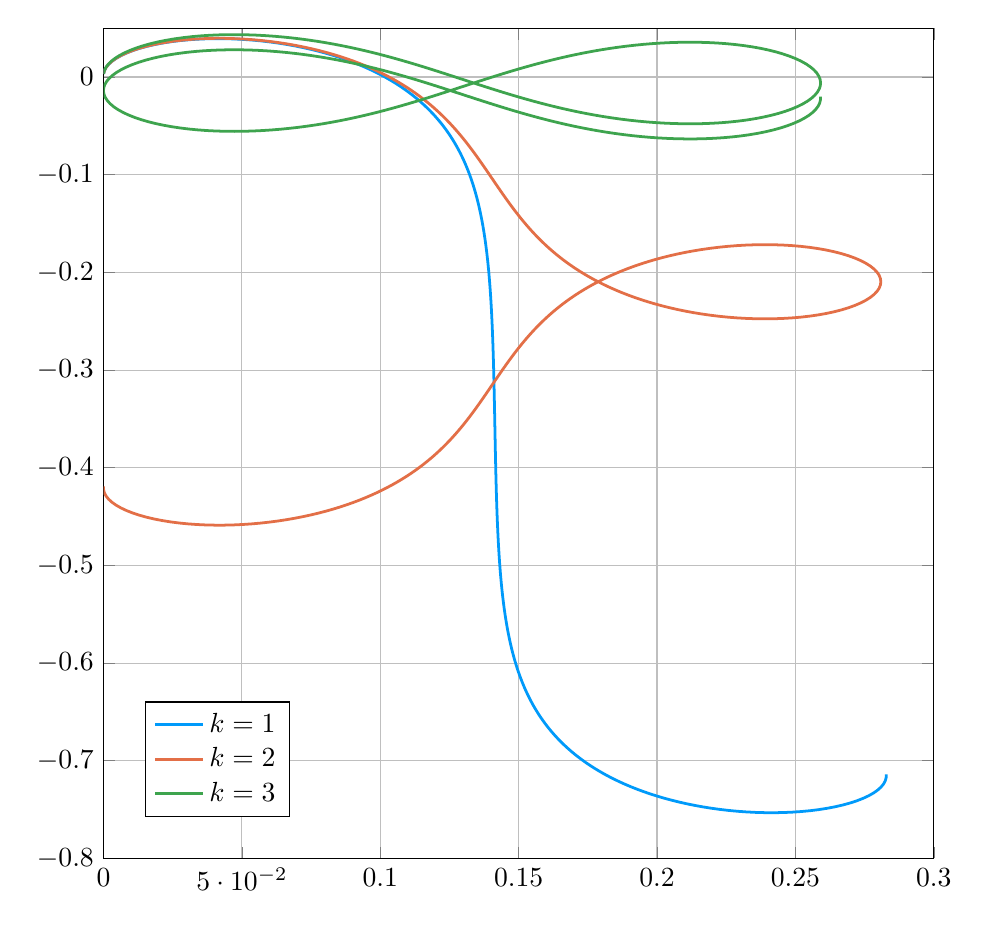
\begin{tikzpicture}[]
\begin{axis}[
    width = {\linewidth},
    ymax = {0.05},
    height = {\linewidth},
    xlabel = {},
    legend style={at={(0.05,0.05)},anchor=south west},
    {
        unbounded coords=jump,
        xshift = 0.0mm,
        yshift = 0.0mm,
        axis background/.style={fill={rgb,1:red,1.00000000;green,1.00000000;blue,1.00000000}},
        grid = major
    }, 
    ylabel = {},
    ymin = {-0.8},
    xmax = {0.3},
    xmin = {0}
]
\addplot+ [color = {rgb,1:red,0.00000000;green,0.60560316;blue,0.97868012},
draw opacity=1.0,
line width=1,
solid,mark = none,
mark size = 2.0,
mark options = {
    color = {rgb,1:red,0.00000000;green,0.00000000;blue,0.00000000}, draw opacity = 1.0,
    fill = {rgb,1:red,0.00000000;green,0.60560316;blue,0.97868012}, fill opacity = 1.0,
    line width = 1,
    rotate = 0,
    solid
}]coordinates {
(0.0, 0.0033222591362126247)
(0.00031166676494506665, 0.006629866972062717)
(0.0009315754659913689, 0.009893778577868753)
(0.0018529678391422083, 0.013085712452943193)
(0.003065930463094352, 0.016178628138997918)
(0.004557651256726709, 0.019147158893764175)
(0.006312742045374353, 0.021967985384662266)
(0.00831361246673031, 0.024620139853220063)
(0.010540878958846471, 0.027085234119418586)
(0.012973792129889028, 0.029347608816571096)
(0.015590666386956994, 0.03139440506701793)
(0.01836929715117594, 0.03321556317225874)
(0.02128735310270589, 0.03480375561396374)
(0.024322733447958027, 0.03615426363978413)
(0.027453882947089718, 0.03726480791275824)
(0.03066006016985871, 0.038135344175268635)
(0.033921556987723894, 0.03876783470895553)
(0.03721986953240519, 0.03916600568447513)
(0.0405378226776505, 0.039335099428017085)
(0.0438596514986479, 0.03928162932291841)
(0.04717104413713541, 0.039013143640024485)
(0.05045915108305971, 0.03853800315520702)
(0.05371256612770184, 0.037865176048555896)
(0.056921284210555374, 0.03700405234494708)
(0.060076641137551914, 0.03596427908533555)
(0.06317123975320013, 0.034755616528549575)
(0.06619886665895634, 0.03338781497580543)
(0.06915440303112388, 0.03187051127484673)
(0.07203373254081716, 0.03021314368050995)
(0.07483364884385643, 0.028424883502537208)
(0.07755176460936235, 0.02651458183697324)
(0.08018642360463508, 0.024490729632197228)
(0.08273661695717152, 0.022361429363839756)
(0.08520190437445938, 0.020134376666144777)
(0.08758234081729148, 0.017816850375078144)
(0.08987840888934118, 0.015415709567740462)
(0.09209095701983042, 0.012937396323128942)
(0.09422114337179528, 0.01038794307310634)
(0.09627038529997763, 0.007772983553739407)
(0.0982403141041456, 0.005097766501861631)
(0.1001327347704296, 0.002367171367102634)
(0.10194959036030368, -0.00041427457587226736)
(0.10369293068996077, -0.003242378227285943)
(0.10536488493841141, -0.006113262195550101)
(0.10696763782762878, -0.00902334620537759)
(0.10850340902993294, -0.01196932865310559)
(0.1099744354744873, -0.0149481685225128)
(0.11138295624461396, -0.01795706782429578)
(0.11273119977931496, -0.020993454680295055)
(0.11402137311490798, -0.024054967138586392)
(0.11525565292528346, -0.027139437776775008)
(0.11643617814141237, -0.030244879127409734)
(0.11756504395197692, -0.03336946994060219)
(0.11864429700710152, -0.03651154228400113)
(0.11967593166595628, -0.03966956946862097)
(0.12066188714640746, -0.042842154780116395)
(0.12160404545086592, -0.04602802098846354)
(0.12250422995705176, -0.049226000604247734)
(0.12336420457559455, -0.05243502684652286)
(0.12418567338828854, -0.05565412528520401)
(0.12497028069150116, -0.05888240611993536)
(0.12571961137877682, -0.0621190570571319)
(0.12643519160517475, -0.06536333674725366)
(0.12711848968342246, -0.06861456874519094)
(0.1277709171686391, -0.07187213595780255)
(0.12839383009427174, -0.07513547554405894)
(0.1289885303270729, -0.07840407423482147)
(0.129556267013497, -0.081677464040976)
(0.13009823809388527, -0.08495521832038302)
(0.13061559186429292, -0.0882369481758698)
(0.13110942856885818, -0.09152229915824175)
(0.13158080200826064, -0.09481094825000788)
(0.132030721152121, -0.09810260110718104)
(0.1324601517451909, -0.10139698953811688)
(0.13287001789891167, -0.10469386919988531)
(0.13326120366141422, -0.10799301749412181)
(0.13363455456032014, -0.11129423164567792)
(0.1339908791138114, -0.114597326948682)
(0.13433095030638684, -0.11790213516582994)
(0.13465550702653503, -0.12120850306785699)
(0.13496525546424865, -0.12451629110119321)
(0.13526087046689378, -0.12782537217278384)
(0.13554299685244825, -0.13113563054196323)
(0.13581225067954372, -0.13444696081010965)
(0.13606922047410236, -0.1377592669995844)
(0.13631446841265238, -0.14107246171417412)
(0.1365485314626544, -0.14438646537391442)
(0.13677192248037068, -0.14770120551777968)
(0.1369851312669764, -0.15101661616828171)
(0.13718862558374248, -0.15433263725253196)
(0.13738285212722734, -0.15764921407479227)
(0.13756823746549504, -0.16096629683597014)
(0.13774518893644155, -0.16428384019590958)
(0.13791409550935366, -0.16760180287468932)
(0.1380753286108587, -0.17092014728947322)
(0.13822924291643965, -0.1742388392237578)
(0.13837617710870118, -0.17755784752614162)
(0.1385164546035706, -0.1808771438359913)
(0.13865038424561216, -0.18419670233361274)
(0.13877826097362062, -0.18751649951274615)
(0.1389003664576416, -0.1908365139733954)
(0.13901696970854724, -0.1941567262331804)
(0.1391283276612696, -0.19747711855555947)
(0.13923468573276945, -0.2007976747934171)
(0.1393362783557891, -0.2041183802466448)
(0.13943332948940826, -0.20743922153246552)
(0.13952605310739288, -0.2107601864673626)
(0.13961465366529413, -0.21408126395957622)
(0.13969932654722522, -0.21740244391122202)
(0.13978025849321118, -0.2207237171291713)
(0.13985762800797713, -0.22404507524390885)
(0.1399316057520084, -0.22736651063565388)
(0.1400023549156869, -0.23068801636709357)
(0.14007003157727826, -0.23400958612213776)
(0.14013478504551438, -0.23733121415015349)
(0.14019675818749008, -0.24065289521518995)
(0.14025608774256268, -0.24397462454974495)
(0.14031290462291882, -0.24729639781266563)
(0.1403673342014464, -0.2506182110508128)
(0.14041949658752473, -0.25394006066414976)
(0.14046950689132284, -0.2572619433739488)
(0.14051747547717242, -0.2605838561938344)
(0.14056350820656022, -0.2639057964034067)
(0.14060770667126388, -0.26722776152421485)
(0.1406501684171348, -0.27054974929786574)
(0.14069098715901232, -0.27387175766607613)
(0.14073025298723588, -0.27719378475249223)
(0.1407680525662032, -0.2805158288461156)
(0.14080446932540724, -0.2838378883861897)
(0.14083958364336768, -0.2871599619484129)
(0.1408734730248585, -0.2904820482323571)
(0.14090621227181885, -0.29380414604998034)
(0.14093787364832078, -0.2971262543151316)
(0.14096852703995483, -0.3004483720339564)
(0.14099824010798317, -0.30377049829611685)
(0.14102707843859752, -0.3070926322667502)
(0.14105510568760957, -0.3104147731790929)
(0.14108238372089194, -0.3137369203277075)
(0.1411089727508774, -0.3170590730622507)
(0.14113493146941725, -0.3203812307817276)
(0.14116031717728983, -0.32370339292918276)
(0.1411851859106452, -0.32702555898677976)
(0.14120959256466317, -0.3303477284712263)
(0.14123359101469787, -0.33366990092950477)
(0.14125723423517464, -0.33699207593487)
(0.14128057441650163, -0.34031425308307933)
(0.14130366308025352, -0.3436364319888209)
(0.1413265511928813, -0.3469586122823102)
(0.14134928927819798, -0.3502807936060227)
(0.1413719275288893, -0.35360297561153564)
(0.14139451591729404, -0.3569251579564495)
(0.14141710430569876, -0.3602473403013634)
(0.1414397425563901, -0.36356952230687634)
(0.14146248064170677, -0.3668917036305889)
(0.1414853687543345, -0.37021388392407817)
(0.14150845741808643, -0.3735360628298197)
(0.14153179759941342, -0.37685823997802903)
(0.1415554408198902, -0.3801804149833943)
(0.1415794392699249, -0.3835025874416728)
(0.14160384592394287, -0.38682475692611934)
(0.14162871465729823, -0.39014692298371634)
(0.14165410036517082, -0.3934690851311715)
(0.14168005908371065, -0.3967912428506485)
(0.14170664811369615, -0.4001133955851916)
(0.14173392614697847, -0.4034355427338063)
(0.14176195339599051, -0.40675768364614895)
(0.14179079172660486, -0.4100798176167822)
(0.14182050479463323, -0.41340194387894275)
(0.1418511581862673, -0.41672406159776754)
(0.14188281956276919, -0.42004616986291876)
(0.14191555880972953, -0.423368267680542)
(0.14194944819122038, -0.4266903539644862)
(0.14198456250918082, -0.43001242752670943)
(0.14202097926838486, -0.43333448706678357)
(0.14205877884735219, -0.4366565311604069)
(0.14209804467557574, -0.43997855824682297)
(0.14213886341745327, -0.4433005666150334)
(0.14218132516332416, -0.4466225543886842)
(0.14222552362802784, -0.44994451950949244)
(0.14227155635741565, -0.45326645971906476)
(0.14231952494326522, -0.45658837253895024)
(0.14236953524706333, -0.45991025524874934)
(0.14242169763314166, -0.4632321048620863)
(0.14247612721166925, -0.4665539181002335)
(0.14253294409202538, -0.4698756913631542)
(0.14259227364709795, -0.4731974206977092)
(0.14265424678907368, -0.4765191017627457)
(0.1427190002573098, -0.4798407297907614)
(0.14278667691890115, -0.48316229954580553)
(0.14285742608257967, -0.4864838052772452)
(0.14293140382661093, -0.4898052406689902)
(0.14300877334137688, -0.49312659878372783)
(0.14308970528736284, -0.4964478720016771)
(0.1431743781692939, -0.49976905195332294)
(0.14326297872719518, -0.5030901294455364)
(0.1433557023451798, -0.5064110943804335)
(0.14345275347879896, -0.5097319356662543)
(0.14355434610181858, -0.513052641119482)
(0.1436607041733185, -0.5163731973573397)
(0.14377206212604085, -0.5196935896797188)
(0.14388866537694645, -0.5230138019395038)
(0.14401077086096742, -0.5263338164001529)
(0.14413864758897588, -0.5296536135792864)
(0.14427257723101747, -0.5329731720769079)
(0.14441285472588689, -0.5362924683867575)
(0.1445597889181484, -0.5396114766891413)
(0.14471370322372937, -0.5429301686234259)
(0.14487493632523438, -0.5462485130382098)
(0.1450438428981465, -0.5495664757169896)
(0.14522079436909302, -0.552884019076929)
(0.14540617970736072, -0.5562011018381069)
(0.14560040625084555, -0.5595176786603672)
(0.14580390056761164, -0.5628336997446174)
(0.14601710935421736, -0.5661491103951195)
(0.14624050037193367, -0.5694638505389847)
(0.14647456342193566, -0.572777854198725)
(0.1467198113604857, -0.5760910489133148)
(0.1469767811550443, -0.5794033551027895)
(0.1472460349821398, -0.582714685370936)
(0.14752816136769425, -0.5860249437401153)
(0.14782377637033942, -0.5893340248117059)
(0.14813352480805303, -0.5926418128450421)
(0.1484580815282012, -0.5959481807470692)
(0.14879815272077662, -0.5992529889642172)
(0.14915447727426792, -0.6025560842672213)
(0.1495278281731738, -0.6058572984187773)
(0.14991901393567636, -0.6091564467130138)
(0.15032888008939713, -0.6124533263747823)
(0.15075831068246703, -0.6157477148057181)
(0.1512082298263274, -0.6190393676628914)
(0.15167960326572985, -0.6223280167546574)
(0.1521734399702951, -0.6256133677370294)
(0.15269079374070277, -0.6288950975925162)
(0.15323276482109102, -0.6321728518719232)
(0.15380050150751512, -0.6354462416780777)
(0.15439520174031626, -0.6387148403688403)
(0.15501811466594892, -0.6419781799550967)
(0.15567054215116552, -0.6452357471677083)
(0.15635384022941323, -0.6484869791656456)
(0.15706942045581115, -0.6517312588557673)
(0.15781875114308683, -0.6549679097929638)
(0.15860335844629944, -0.6581961906276952)
(0.15942482725899343, -0.6614152890663764)
(0.16028480187753621, -0.6646243153086514)
(0.16118498638372206, -0.6678222949244357)
(0.1621271446881805, -0.6710081611327827)
(0.1631131001686317, -0.6741807464442783)
(0.16414473482748643, -0.677338773628898)
(0.16522398788261103, -0.680480845972297)
(0.16635285369317557, -0.6836054367854895)
(0.16753337890930448, -0.6867108781361242)
(0.16876765871968, -0.6897953487743128)
(0.170057832055273, -0.6928568612326041)
(0.171406075589974, -0.6958932480886034)
(0.17281459636010066, -0.6989021473903864)
(0.17428562280465504, -0.7018809872597935)
(0.1758213940069592, -0.7048269697075217)
(0.17742414689617658, -0.7077370537173491)
(0.17909610114462718, -0.7106079376856133)
(0.18083944147428427, -0.7134360413370269)
(0.18265629706415837, -0.7162174872800018)
(0.18454871773044235, -0.7189480824147608)
(0.1865186465346103, -0.7216232994666386)
(0.18856788846279268, -0.7242382589860056)
(0.19069807481475756, -0.7267877122360281)
(0.1929106229452468, -0.7292660254806397)
(0.19520669101729649, -0.7316671662879773)
(0.1975871274601286, -0.733984692579044)
(0.20005241487741643, -0.7362117452767389)
(0.20260260822995288, -0.7383410455450964)
(0.2052372672252256, -0.7403648977498724)
(0.20795538299073155, -0.7422751994154364)
(0.21075529929377082, -0.7440634595934091)
(0.21363462880346407, -0.7457208271877459)
(0.21659016517563165, -0.7472381308887046)
(0.21961779208138785, -0.7486059324414488)
(0.22271239069703602, -0.7498145949982348)
(0.22586774762403258, -0.7508543682578462)
(0.2290764657068861, -0.751715491961455)
(0.23232988075152824, -0.7523883190681062)
(0.23561798769745257, -0.7528634595529237)
(0.23892938033594005, -0.7531319452358176)
(0.24225120915693743, -0.7531854153409163)
(0.24556916230218276, -0.7530163215973743)
(0.24886747484686408, -0.7526181506218548)
(0.2521289716647293, -0.7519856600881678)
(0.25533514888749825, -0.7511151238256575)
(0.25846629838662993, -0.7500045795526833)
(0.26150167873188207, -0.7486540715268629)
(0.26441973468341207, -0.7470658790851579)
(0.267198365447631, -0.7452447209799171)
(0.26981523970469895, -0.7431979247294702)
(0.2722481528757415, -0.7409355500323177)
(0.2744754193678577, -0.7384704557661192)
(0.2764762897892136, -0.7358183012975614)
(0.2782313805778613, -0.7329974748066633)
(0.27972310137149364, -0.7300289440518971)
(0.2809360639954458, -0.7269360283658424)
(0.2818574563685966, -0.7237440944907679)
(0.2824773650696429, -0.720480182884962)
(0.282789031834588, -0.7171725750491118)
(0.282789031834588, -0.7138503159128992)
};
\addlegendentry{$k = 1$}
\addplot+ [color = {rgb,1:red,0.88887350;green,0.43564919;blue,0.27812294},
draw opacity=1.0,
line width=1,
solid,mark = none,
mark size = 2.0,
mark options = {
    color = {rgb,1:red,0.00000000;green,0.00000000;blue,0.00000000}, draw opacity = 1.0,
    fill = {rgb,1:red,0.88887350;green,0.43564919;blue,0.27812294}, fill opacity = 1.0,
    line width = 1,
    rotate = 0,
    solid
}]coordinates {
(0.0, 0.0033222591362126247)
(0.0003095114856480428, 0.00663006934969226)
(0.0009251708545573729, 0.009894785158093111)
(0.0018403401131212307, 0.013088508846255243)
(0.003045280927290875, 0.01618455849096323)
(0.004527405111238953, 0.019157892254855955)
(0.0062715897660642434, 0.021985475261245026)
(0.008260542769846049, 0.024646578738544544)
(0.010475202822581986, 0.027123004917327977)
(0.012895157800708256, 0.029399235062104675)
(0.015499065715045513, 0.03146250172974607)
(0.018265063951972832, 0.03330278962066511)
(0.02117115451342228, 0.03491277204814768)
(0.024195555431752613, 0.03628769199249021)
(0.027317011193999385, 0.037425197901259345)
(0.03051505766037986, 0.03832514488137519)
(0.03377023943465186, 0.03898937178883654)
(0.03706427981443022, 0.03942146407589782)
(0.040380205240327545, 0.03962651123641437)
(0.04370242753996523, 0.039610866430937926)
(0.04701678822936941, 0.03938191449563163)
(0.05031056972074367, 0.03894785314601776)
(0.05357247854140008, 0.03831749085822433)
(0.05679260565307272, 0.03750006370378236)
(0.05996236873617785, 0.03650507236455772)
(0.06307444092957591, 0.03534213967896201)
(0.06612267004664578, 0.0340208883713011)
(0.06910199176840215, 0.03255083808426363)
(0.0720083397803541, 0.030941320454173436)
(0.07483855529933274, 0.02920141071965249)
(0.07759029794902177, 0.027339874215033068)
(0.08026195950086214, 0.025365126048667)
(0.08285258160713613, 0.02328520228308502)
(0.08536177831772546, 0.021107741000830852)
(0.08778966389039738, 0.0188399717413691)
(0.09013678617338962, 0.01648871191803404)
(0.09240406565402666, 0.01406036895938292)
(0.09459274012285389, 0.011560947058692254)
(0.09670431479380659, 0.008996057552857898)
(0.09874051764182308, 0.006370932083498802)
(0.10070325966496342, 0.003690437815878143)
(0.10259459974387716, 0.0009590941037022451)
(0.10441671375326944, -0.0018189099108601213)
(0.10617186757429908, -0.004639697182646725)
(0.1078623936605932, -0.00749968447627362)
(0.10949067082127585, -0.010395564179601698)
(0.11105910690003078, -0.01332428643256597)
(0.11257012404810286, -0.016283041736132046)
(0.11402614630998247, -0.019269244164143128)
(0.11542958926230334, -0.02228051526580918)
(0.11678285146844976, -0.025314668717690617)
(0.11808830753294519, -0.028369695760422045)
(0.11934830256048083, -0.031443751436354694)
(0.12056514784415776, -0.03453514162909024)
(0.12174111762599216, -0.03764231089392932)
(0.12287844678986712, -0.04076383105903281)
(0.1239793293628735, -0.04389839057012828)
(0.12504591771536952, -0.04704478454648726)
(0.12608032236314295, -0.05020190551230611)
(0.1270846122868389, -0.053368734765251565)
(0.12806081569439295, -0.0565443343425327)
(0.12901092116166582, -0.059727839544225704)
(0.12993687909489307, -0.06291845197353169)
(0.1308406034660307, -0.066115433054045)
(0.13172397377867442, -0.06931809798483124)
(0.1325888372280362, -0.0725258100950597)
(0.1334370110235535, -0.07573797556102595)
(0.1342702848471496, -0.07895403844956805)
(0.13509042342402328, -0.08217347605307458)
(0.13589916918617895, -0.08539579448245793)
(0.13669824501176447, -0.08862052448559199)
(0.1374893570257092, -0.09184721745975928)
(0.1382741974491872, -0.0950754416275988)
(0.1390544474871056, -0.0983047783468767)
(0.13983178024416007, -0.10153481852510333)
(0.14060786366103623, -0.10476515911058316)
(0.14138436346308011, -0.1079953996319026)
(0.14216294611422958, -0.11122513875812895)
(0.14294528176919774, -0.11445397085210872)
(0.1437330472168326, -0.11768148248921569)
(0.1445279288072453, -0.12090724891370633)
(0.14533162535469216, -0.12413083040449734)
(0.14614585100730934, -0.12735176852168745)
(0.1469723380736102, -0.130569582204514)
(0.1478128397941506, -0.13378376369066516)
(0.1486691330449185, -0.13699377422598083)
(0.14954302095677816, -0.14019903953257462)
(0.15043633543266557, -0.14339894500232184)
(0.15135093954114145, -0.14659283058150394)
(0.1522887297613204, -0.14977998531120956)
(0.15325163805004885, -0.1529596414869063)
(0.15424163369744753, -0.1561309683994588)
(0.1552607249314923, -0.15929306561884368)
(0.15631096022611635, -0.16244495578096452)
(0.15739442926029543, -0.16558557683739958)
(0.15851326346764447, -0.1687137737277206)
(0.15966963610712873, -0.17182828943434342)
(0.16086576177548667, -0.17492775538086447)
(0.16210389527079225, -0.17801068113669294)
(0.16338632970417752, -0.18107544339373932)
(0.16471539374302085, -0.1841202741852287)
(0.1660934478538365, -0.18714324832269866)
(0.16752287939665292, -0.19014227003528256)
(0.16900609640485428, -0.1931150588059036)
(0.17054551986534797, -0.19605913441251255)
(0.17214357429364205, -0.19897180119955804)
(0.1738026763771938, -0.20185013162612525)
(0.17552522143856017, -0.2046909491633336)
(0.17731356744792195, -0.20749081064543376)
(0.17917001629313137, -0.21024598821743684)
(0.18109679199542636, -0.21295245106794744)
(0.18309601554151902, -0.21560584719007037)
(0.18516967598936665, -0.21820148547673135)
(0.1873195974974194, -0.22073431853032185)
(0.18954740192777625, -0.22319892665094276)
(0.19185446668522838, -0.22558950356312746)
(0.19424187747989394, -0.22789984454784432)
(0.1967103757448874, -0.2301233377643558)
(0.19926030050658192, -0.23225295967395512)
(0.20189152459840026, -0.23428127561255618)
(0.20460338523498894, -0.23620044669817333)
(0.2073946091275883, -0.23800224439756437)
(0.2102632325288493, -0.23967807420690845)
(0.2132065168512157, -0.24121901001538987)
(0.2162208608111939, -0.242615840806535)
(0.21930171041448787, -0.24385913139607218)
(0.22244346851348185, -0.2449392988902849)
(0.2256394061345031, -0.2458467064562053)
(0.22888157827824035, -0.24657177580359385)
(0.2321607474268571, -0.24710511946663677)
(0.23546631852237385, -0.2474376935194921)
(0.2387862896809241, -0.2475609707458674)
(0.2421072233355875, -0.2474671334959496)
(0.24541424280698695, -0.24714928450046075)
(0.24869105942867697, -0.2466016727803851)
(0.2519200352419814, -0.24581993051771575)
(0.25508228586077986, -0.24480131538330183)
(0.2581578273354861, -0.24354495142110374)
(0.2611257696759538, -0.24205206025567766)
(0.2639645581073342, -0.2403261732344596)
(0.2666522611454438, -0.23837331426692387)
(0.2691669022439825, -0.23620214271366308)
(0.2714868291858861, -0.23382404583750818)
(0.27359111271292713, -0.23125317116028793)
(0.2754599633007228, -0.22850639063599337)
(0.277075152709361, -0.22560319085947592)
(0.27842042520193444, -0.22256548651427152)
(0.2794818823389601, -0.21941735778208707)
(0.28024832519836995, -0.21618471627529917)
(0.2807115388422244, -0.21289490793919574)
(0.2808665058665012, -0.2095762649952298)
(0.2807115388422251, -0.2062576220512638)
(0.28024832519837156, -0.2029678137151603)
(0.27948188233896243, -0.19973517220837222)
(0.27842042520193755, -0.1965870434761875)
(0.2770751527093649, -0.19354933913098277)
(0.27545996330072736, -0.1906461393544649)
(0.27359111271293224, -0.18789935883016992)
(0.27148682918589184, -0.1853284841529492)
(0.26916690224398876, -0.18295038727679377)
(0.2666522611454506, -0.18077921572353242)
(0.26396455810734143, -0.17882635675599615)
(0.2611257696759614, -0.17710046973477744)
(0.258157827335494, -0.17560757856935072)
(0.255082285860788, -0.174351214607152)
(0.25192003524198975, -0.17333259947273755)
(0.24869105942868552, -0.17255085721006755)
(0.24541424280699556, -0.17200324548999132)
(0.2421072233355962, -0.17168539649450187)
(0.2387862896809328, -0.1715915592445835)
(0.2354663185223825, -0.17171483647095823)
(0.23216074742686577, -0.17204741052381303)
(0.22888157827824887, -0.1725807541868554)
(0.2256394061345115, -0.17330582353424348)
(0.22244346851349017, -0.1742132311001634)
(0.21930171041449598, -0.17529339859437568)
(0.2162208608112019, -0.17653668918391244)
(0.2132065168512235, -0.17793351997505719)
(0.2102632325288569, -0.17947445578353827)
(0.2073946091275957, -0.18115028559288196)
(0.20460338523499616, -0.18295208329227272)
(0.20189152459840726, -0.1848712543778896)
(0.1992603005065887, -0.18689957031649032)
(0.19671037574489397, -0.1890291922260894)
(0.1942418774799003, -0.19125268544260063)
(0.1918544666852345, -0.1935630264273173)
(0.1895474019277822, -0.19595360333950182)
(0.18731959749742508, -0.1984182114601225)
(0.18516967598937217, -0.20095104451371285)
(0.18309601554152433, -0.20354668280037372)
(0.18109679199543147, -0.2062000789224965)
(0.17917001629313628, -0.20890654177300694)
(0.1773135674479267, -0.2116617193450099)
(0.17552522143856472, -0.21446158082710992)
(0.17380267637719815, -0.2173023983643182)
(0.17214357429364624, -0.2201807287908853)
(0.17054551986535202, -0.22309339557793073)
(0.16900609640485817, -0.22603747118453957)
(0.16752287939665664, -0.2290102599551605)
(0.1660934478538401, -0.23200928166774437)
(0.16471539374302427, -0.23503225580521428)
(0.1633863297041808, -0.23807708659670354)
(0.1621038952707954, -0.2411418488537499)
(0.16086576177548967, -0.2442247746095783)
(0.15966963610713164, -0.2473242405560993)
(0.15851326346764724, -0.2504387562627221)
(0.1573944292602981, -0.25356695315304306)
(0.15631096022611887, -0.2567075742094781)
(0.15526072493149473, -0.2598594643715989)
(0.1542416336974499, -0.2630215615909837)
(0.15325163805005113, -0.26619288850353623)
(0.15228872976132257, -0.2693725446792329)
(0.15135093954114356, -0.2725596994089385)
(0.15043633543266757, -0.2757535849881206)
(0.1495430209567801, -0.2789534904578678)
(0.14866913304492035, -0.2821587557644616)
(0.14781283979415238, -0.28536876629977725)
(0.1469723380736119, -0.28858294778592836)
(0.14614585100731098, -0.2918007614687549)
(0.1453316253546937, -0.295021699585945)
(0.1445279288072468, -0.298245281076736)
(0.14373304721683408, -0.30147104750122666)
(0.14294528176919916, -0.30469855913833355)
(0.14216294611423094, -0.30792739123231333)
(0.1413843634630814, -0.31115713035853965)
(0.1406078636610375, -0.3143873708798591)
(0.1398317802441613, -0.3176177114653389)
(0.13905444748710677, -0.3208477516435655)
(0.13827419744918837, -0.32407708836284344)
(0.1374893570257103, -0.3273053125306829)
(0.13669824501176556, -0.33053200550485023)
(0.13589916918617997, -0.33375673550798424)
(0.13509042342402428, -0.33697905393736755)
(0.13427028484715056, -0.3401984915408741)
(0.13343701102355443, -0.3434145544294162)
(0.13258883722803708, -0.34662671989538246)
(0.1317239737786753, -0.3498344320056109)
(0.13084060346603157, -0.3530370969363971)
(0.12993687909489393, -0.3562340780169104)
(0.12901092116166665, -0.35942469044621644)
(0.12806081569439373, -0.3626081956479094)
(0.12708461228683968, -0.3657837952251905)
(0.12608032236314376, -0.368950624478136)
(0.1250459177153703, -0.3721077454439548)
(0.12397932936287423, -0.3752541394203138)
(0.12287844678986783, -0.37838869893140925)
(0.12174111762599284, -0.3815102190965128)
(0.12056514784415845, -0.38461738836135184)
(0.11934830256048151, -0.38770877855408736)
(0.11808830753294587, -0.39078283423002)
(0.11678285146845041, -0.3938378612727514)
(0.11542958926230401, -0.39687201472463285)
(0.11402614630998309, -0.39988328582629895)
(0.1125701240481035, -0.40286948825431)
(0.11105910690003142, -0.40582824355787606)
(0.10949067082127649, -0.40875696581084037)
(0.10786239366059382, -0.4116528455141684)
(0.10617186757429968, -0.41451283280779533)
(0.10441671375327005, -0.4173336200795819)
(0.10259459974387776, -0.42011162409414426)
(0.10070325966496402, -0.42284296780632014)
(0.09874051764182366, -0.4255234620739408)
(0.09670431479380719, -0.42814858754329993)
(0.09459274012285446, -0.43071347704913426)
(0.09240406565402726, -0.43321289894982495)
(0.0901367861733902, -0.4356412419084761)
(0.08778966389039797, -0.4379925017318111)
(0.08536177831772604, -0.44026027099127285)
(0.08285258160713671, -0.44243773227352706)
(0.0802619595008627, -0.444517656039109)
(0.07759029794902234, -0.44649240420547504)
(0.07483855529933332, -0.4483539407100945)
(0.07200833978035469, -0.4500938504446154)
(0.06910199176840273, -0.45170336807470574)
(0.06612267004664638, -0.45317341836174313)
(0.0630744409295765, -0.45449466966940405)
(0.05996236873617844, -0.4556576023549997)
(0.05679260565307331, -0.45665259369422434)
(0.05357247854140067, -0.45747002084866634)
(0.05031056972074426, -0.4581003831364598)
(0.047016788229370006, -0.45853444448607367)
(0.04370242753996583, -0.45876339642138)
(0.040380205240328156, -0.45877904122685653)
(0.037064279814430834, -0.45857399406633986)
(0.03377023943465247, -0.4581419017792786)
(0.030515057660380478, -0.4574776748718173)
(0.027317011194000006, -0.4565777278917015)
(0.024195555431753227, -0.4554402219829323)
(0.021171154513422892, -0.4540653020385898)
(0.018265063951973436, -0.4524553196111073)
(0.015499065715046124, -0.45061503172018824)
(0.012895157800708873, -0.4485517650525468)
(0.010475202822582595, -0.4462755349077701)
(0.008260542769846661, -0.4437991087289867)
(0.006271589766064856, -0.4411380052516871)
(0.004527405111239561, -0.4383104222452981)
(0.0030452809272914915, -0.43533708848140534)
(0.0018403401131218467, -0.4322410388366974)
(0.0009251708545579844, -0.4290473151485353)
(0.0003095114856486627, -0.42578259934013435)
(6.137578448426114e-16, -0.42247478912665476)
(6.137578448426114e-16, -0.4191525299904421)
};
\addlegendentry{$k = 2$}
\addplot+ [color = {rgb,1:red,0.24222430;green,0.64327509;blue,0.30444865},
draw opacity=1.0,
line width=1,
solid,mark = none,
mark size = 2.0,
mark options = {
    color = {rgb,1:red,0.00000000;green,0.00000000;blue,0.00000000}, draw opacity = 1.0,
    fill = {rgb,1:red,0.24222430;green,0.64327509;blue,0.30444865}, fill opacity = 1.0,
    line width = 1,
    rotate = 0,
    solid
}]coordinates {
(-0.0, 0.0033222591362126247)
(0.00028558339580241353, 0.006632221053242821)
(0.0008540149211008802, 0.009905490270584271)
(0.0016998916546389407, 0.013118261398412588)
(0.0028152751818666896, 0.01624769031681563)
(0.004189882405913294, 0.019272233381106032)
(0.005811326686000462, 0.022171944438215147)
(0.007665399134373894, 0.02492872174592986)
(0.009736378727460589, 0.027526499506471888)
(0.012007359417917229, 0.02995138145653076)
(0.014460582644684604, 0.03219171660284198)
(0.0170777644484493, 0.03423811958715158)
(0.019840407691242738, 0.036083440177508724)
(0.022730091509612554, 0.037722687931205486)
(0.025728731952735902, 0.039152919122661355)
(0.028818809629827767, 0.04037309358464898)
(0.031983561994098936, 0.041383909216200214)
(0.03520713952829842, 0.042187621633145884)
(0.03847472650360679, 0.042787855859880194)
(0.04177262812204757, 0.043189416170710225)
(0.04508832671092227, 0.04339809926988841)
(0.04841051022512407, 0.043420515025821324)
(0.05172907665393798, 0.04326391800893555)
(0.05503511805734145, 0.04293605217184628)
(0.05832088791208716, 0.04244501018810903)
(0.06157975527012775, 0.0417991082521731)
(0.06480614895931819, 0.04100677654732948)
(0.06799549472282211, 0.04007646511078371)
(0.0711441478280722, 0.03901656445933222)
(0.07424932330169176, 0.03783534007498357)
(0.07730902558117272, 0.036540879674242285)
(0.0803219790299831, 0.03514105208362625)
(0.08328756044843999, 0.033643476503346086)
(0.08620573443282616, 0.032055500947803725)
(0.08907699219170441, 0.030384188693845876)
(0.09190229422092291, 0.0286363116352854)
(0.09468301706562837, 0.026818349526471958)
(0.09742090425595198, 0.02493649419164673)
(0.10011802138957421, 0.022996657874925726)
(0.10277671524553164, 0.021004485003801712)
(0.1053995767458091, 0.018965366733933467)
(0.10798940753102, 0.01688445773252994)
(0.11054918988062498, 0.014766694740408527)
(0.1130820596837971, 0.012616816527967863)
(0.11559128215166885, 0.0104393849274633)
(0.11808022995309855, 0.008238806683022432)
(0.12055236345240128, 0.006019355910922823)
(0.12301121272714229, 0.0037851970060429818)
(0.12546036104580993, 0.0015404078664319398)
(0.12790342948793906, -0.0007109966630165399)
(0.13034406239224267, -0.0029650412044084683)
(0.13278591332092518, -0.005217766178798509)
(0.13523263123016951, -0.0074652041069138)
(0.1376878465375591, -0.009703355925381007)
(0.14015515677680804, -0.011928167367154362)
(0.14263811152868372, -0.014135505462754166)
(0.14514019631461716, -0.016321135232900224)
(0.14766481513657542, -0.01848069666336759)
(0.15021527134386042, -0.02060968207967969)
(0.15279474650533095, -0.022703414072916855)
(0.1554062769650746, -0.024757024168816102)
(0.15805272776197432, -0.026765432480822693)
(0.16073676360038502, -0.02872332864412536)
(0.16346081657202308, -0.030625154392152264)
(0.16622705035025845, -0.032465088209521216)
(0.16903732060971144, -0.0342370325757422)
(0.17189313146916113, -0.03593460440137947)
(0.1747955878173604, -0.03755112935168061)
(0.17774534346279303, -0.03907964084996466)
(0.18074254515326005, -0.040512884651559465)
(0.18378677264304805, -0.04184332997496336)
(0.18687697514775878, -0.04306318826510522)
(0.19001140472265543, -0.04416444073759343)
(0.19318754733176824, -0.045138875904614)
(0.19640205264283525, -0.04597813830295561)
(0.19965066388636496, -0.04667378962118956)
(0.20292814945202786, -0.04721738334357756)
(0.20622823825520997, -0.04760055387905791)
(0.20954356127976498, -0.047815120910550755)
(0.2128656020738336, -0.047853209369333155)
(0.21618465932272413, -0.04770738499984926)
(0.2194898249193067, -0.04737080492421315)
(0.22276898116579127, -0.04683738194074743)
(0.22600882083423454, -0.04610196050311481)
(0.2291948937469024, -0.04516050144223522)
(0.23231168327178808, -0.044010271540993115)
(0.23534271562674103, -0.042650033094478526)
(0.2382707041195344, -0.0410802276434057)
(0.24107772940598188, -0.039303147226150276)
(0.24374545552813306, -0.03732308583686444)
(0.24625537992793783, -0.03514646339017947)
(0.2485891138747633, -0.03278191446203639)
(0.25072868788324737, -0.030240334475026793)
(0.25265687484419697, -0.02753487687754497)
(0.25435752188045446, -0.024680896249331653)
(0.25581588051881343, -0.021695834131037955)
(0.25701892378375757, -0.018599046655149304)
(0.2579556383973, -0.015411575635528214)
(0.25861728050591926, -0.012155867496236527)
(0.2589975842962206, -0.00885544709949452)
(0.2590929144919073, -0.005534555965786792)
(0.25890235596885847, -0.002217766370795622)
(0.25842773644558314, 0.001070415813371521)
(0.2576735812175489, 0.004305946011063515)
(0.25664700198999985, 0.007465620180612175)
(0.2553575248011113, 0.010527425913751437)
(0.25381686460757613, 0.013470854515943874)
(0.25203865615693816, 0.016277165345881972)
(0.2500381521772588, 0.01892959623007769)
(0.247831900619125, 0.021413516484510297)
(0.24543741269456784, 0.023716521770500328)
(0.24287283283553368, 0.025828472507327477)
(0.24015662054861217, 0.027741479716023948)
(0.23730725260867896, 0.029449843878323403)
(0.23434295225968954, 0.030949953610686136)
(0.231281450220305, 0.032240151669509984)
(0.2281397804538239, 0.03332057605211471)
(0.22493411196028737, 0.03419298379949857)
(0.2216796163593647, 0.03486056461986654)
(0.21839036980230137, 0.03532775072303652)
(0.21507928679960964, 0.035600028370731326)
(0.21175808287557216, 0.03568375568471179)
(0.2084372625411036, 0.03558599028015441)
(0.2051261288815309, 0.03531432935806032)
(0.20183281104735865, 0.03487676403576957)
(0.19856430607386172, 0.0342815489432407)
(0.19532653170034966, 0.03353708747722859)
(0.19212438717663488, 0.03265183258885375)
(0.1889618194019808, 0.03163420257806008)
(0.1858418921155257, 0.03049251107183737)
(0.18276685622737487, 0.02923491015949172)
(0.17973821973196305, 0.027869345533848577)
(0.17675681597023632, 0.026403522427975997)
(0.17382286929888513, 0.024844881129339375)
(0.17093605748055699, 0.023200580884946878)
(0.16809557032832345, 0.021477491071227216)
(0.1653001643220139, 0.01968218858194121)
(0.16254821306583814, 0.017820960478838004)
(0.159837753579187, 0.01589981104702095)
(0.15716652850914356, 0.013924472495450702)
(0.15453202442767563, 0.011900418639231185)
(0.15193150643220893, 0.009832880991834622)
(0.14936204930859437, 0.007726866780568537)
(0.14682056554336254, 0.0055871784763496125)
(0.14430383049025955, 0.0034184344986908804)
(0.141808505006692, 0.0012250908185516853)
(0.13933115588084735, -0.0009885367645853396)
(0.13686827437156387, -0.0032182498491273017)
(0.13441629318186646, -0.005459944300545334)
(0.13197160218457757, -0.007709586871249171)
(0.12953056321542447, -0.009963191654529559)
(0.12708952424627137, -0.012216796437809952)
(0.12464483324898253, -0.014466439008513797)
(0.12219285205928515, -0.016708133459931843)
(0.11972997055000165, -0.018937846544473825)
(0.11725262142415702, -0.02115147412761087)
(0.11475729594058948, -0.023344817807750093)
(0.11224056088748653, -0.02551356178540886)
(0.10969907712225474, -0.02765325008962782)
(0.10712961999864022, -0.02975926430089395)
(0.10452910200317356, -0.031826801948290566)
(0.10189459792170567, -0.03385085580451013)
(0.09922337285166229, -0.03582619435608045)
(0.09651291336501117, -0.037747343787897576)
(0.09376096210883551, -0.039608571891000866)
(0.09096555610252598, -0.04140387438028696)
(0.0881250689502925, -0.04312696419400672)
(0.08523825713196441, -0.044771264438399315)
(0.0823043104606133, -0.04632990573703605)
(0.07932290669888663, -0.047795728842908745)
(0.07629427020347489, -0.049161293468552025)
(0.0732192343153241, -0.05041889438089782)
(0.07009930702886903, -0.05156058588712068)
(0.06693673925421503, -0.05257821589791451)
(0.06373459473050028, -0.053463470786289526)
(0.06049682035698827, -0.05420793225230182)
(0.05722831538349139, -0.05480314734483089)
(0.053934997549319186, -0.05524071266712184)
(0.05062386388974652, -0.05551237358921614)
(0.047303043555277945, -0.05561013899377373)
(0.04398183963124047, -0.0555264116797935)
(0.04067075662854873, -0.05525413403209893)
(0.03738151007148534, -0.05478694792892921)
(0.03412701447056261, -0.05411936710856149)
(0.030921345977025994, -0.053246959361177904)
(0.027779676210544797, -0.052166534978573424)
(0.02471817417116019, -0.05087633691974984)
(0.021753873822170627, -0.04937622718738738)
(0.018904505882237275, -0.047667863025088186)
(0.016188293595315543, -0.04575485581639196)
(0.013623713736281212, -0.04364290507956506)
(0.011229225811723802, -0.04133989979357526)
(0.009022974253589784, -0.03885597953914287)
(0.0070224702739101474, -0.03620354865494735)
(0.005244261823271851, -0.03339723782500944)
(0.003703601629736402, -0.030453809222817166)
(0.0024141244408475613, -0.02739200348967805)
(0.0013875452132981526, -0.0242323293201295)
(0.000633389985263515, -0.020996799122437584)
(0.00015877046198788043, -0.017708616938270496)
(-3.178806106136132e-5, -0.014391827343279344)
(6.354213462494228e-5, -0.011070936209571607)
(0.00044384592492593755, -0.007770515812829558)
(0.001105488033544831, -0.0045148076735378)
(0.0020422026470869143, -0.0013273366539166072)
(0.0032452459120307113, 0.001769450821972175)
(0.004703604550389346, 0.0047545129402660315)
(0.006404251586646546, 0.007608493568479525)
(0.008332438547595876, 0.010313951165961555)
(0.010472012556079683, 0.012855531152971373)
(0.012805746502904922, 0.015220080081114687)
(0.015315670902709492, 0.017396702527799908)
(0.017983397024860476, 0.019376763917086006)
(0.020790422311307778, 0.0211538443343417)
(0.023718410804100986, 0.0227236497854148)
(0.026749443159053844, 0.02408388823192966)
(0.02986623268393938, 0.02523411813317204)
(0.033052305596607184, 0.0261755771940519)
(0.036292145265050396, 0.02691099863168479)
(0.03957130151153492, 0.027444421615150785)
(0.04287646710811747, 0.027781001690787146)
(0.046195524357008, 0.027926826060271293)
(0.04951756515107659, 0.027888737601489143)
(0.052832888175631615, 0.027674170569996537)
(0.05613297697881376, 0.02729100003451641)
(0.05941046254447669, 0.026747406312128626)
(0.06265907378800645, 0.026051754993894886)
(0.06587357909907353, 0.025212492595553474)
(0.06904972170818638, 0.02423805742853309)
(0.0721841512830831, 0.023136804956045063)
(0.07527435378779389, 0.021916946665903374)
(0.07831858127758197, 0.020586501342499633)
(0.08131578296804906, 0.019153257540904977)
(0.08426553861348177, 0.017624746042621073)
(0.0871679949616811, 0.016008221092320068)
(0.09002380582113086, 0.014310649266682922)
(0.09283407608058393, 0.012538704900462057)
(0.09560030985881937, 0.01069877108309322)
(0.09832436283045752, 0.008796945335066428)
(0.10100839866886827, 0.006839049171763858)
(0.10365484946576806, 0.004830640859757371)
(0.1062663799255118, 0.002777030763858216)
(0.1088458550869824, 0.000683298770621142)
(0.11139631129426747, -0.0014456866456908706)
(0.11392093011622581, -0.0036052480761581554)
(0.11642301490215931, -0.005790877846304132)
(0.11890596965403509, -0.007998215941903863)
(0.12137327989328407, -0.010223027383677148)
(0.12382849520067372, -0.012461179202144285)
(0.12627521310991816, -0.014708617130259513)
(0.12871706403860073, -0.01696134210464949)
(0.1311576969429044, -0.019215386646041357)
(0.13360076538503357, -0.021466791175489774)
(0.13604991370370126, -0.02371158031510076)
(0.1385087629784423, -0.02594573921998055)
(0.1409808964777451, -0.028165189992080102)
(0.14346984427917484, -0.030365768236520926)
(0.1459790667470466, -0.03254319983702544)
(0.1485119365502188, -0.03469307804946605)
(0.15107171889982382, -0.03681084104158741)
(0.15366154968503473, -0.0388917500429909)
(0.15628441118531222, -0.040930868312859095)
(0.15894310504126968, -0.04292304118398306)
(0.16164022217489196, -0.04486287750070403)
(0.16437810936521557, -0.04674473283552922)
(0.16715883220992106, -0.048562694944342615)
(0.1699841342391396, -0.05031057200290305)
(0.1728553919980179, -0.051981884256860865)
(0.17577356598240407, -0.05356985981240319)
(0.17873914740086097, -0.055067435392683314)
(0.18175210084967142, -0.0564672629832993)
(0.18481180312915238, -0.05776172338404054)
(0.18791697860277193, -0.05894294776838915)
(0.19106563170802202, -0.0600028484198406)
(0.19425497747152598, -0.06093315985638634)
(0.19748137116071637, -0.06172549156122994)
(0.200740238518757, -0.062371393497165833)
(0.20402600837350268, -0.06286243548090305)
(0.20733204977690614, -0.06319030131799229)
(0.21065061620572006, -0.06334689833487803)
(0.21397279971992186, -0.06332448257894509)
(0.21728849830879657, -0.06311579947976687)
(0.22058639992723733, -0.06271423916893683)
(0.22385398690254568, -0.062114004942202476)
(0.2270775644367452, -0.061310292525256785)
(0.23024231680101634, -0.06029947689370554)
(0.23333239447810822, -0.059079302431717884)
(0.23633103492123156, -0.05764907124026202)
(0.23922071873960135, -0.05600982348656524)
(0.24198336198239478, -0.05416450289620807)
(0.24460054378615947, -0.05211809991189847)
(0.24705376701292683, -0.049877764765587244)
(0.2493247477033835, -0.04745288281552836)
(0.2513957272964702, -0.044855105054986334)
(0.25324979974484363, -0.04209832774727162)
(0.2548712440249308, -0.039198616690162495)
(0.2562458512489774, -0.036174073625872105)
(0.2573612347762051, -0.03304464470746906)
(0.2582071115097432, -0.029831873579640747)
(0.25877554303504163, -0.02655860436229929)
(0.25906112643084406, -0.023248642445269092)
(0.25906112643084406, -0.01992638330905647)
};
\addlegendentry{$k = 3$}
\end{axis}

\end{tikzpicture}

      \caption{First three non-trivial solutions at $\mu = 200$}
    \end{subfigure}
    \caption{First non-trivial solutions}
    \label{fig:solutions}
  \end{figure}

  \newpage
  \begin{minted}[fontsize=\scriptsize,breaklines=true]{julia}
function buckling_plus_ɛ(θ::Vector{Float64}, μ::Float64, ɛ::Float64, k::Int64)
  n = length(θ);
  h = 1 / (n + 1);
  A = Poisson1D(n);
  rhs = ɛ * sin(k * pi * linspace(h, 1 - h, n));
  return A * θ + (μ * sin(θ) - rhs) * h ^ 2;
end

function ex4_3(; n::Int64 = 1000, k::Int64 = 1, ɛ::Float64 = 0.1, tol::Float64 = 1e-8)
  θ = zeros(n);

  for μ = linspace(0, 50, 100)
    (θ, its) = newton(x -> buckling_plus_ɛ(x, μ, ɛ, k), x -> ∂buckling(x, μ), θ, tol);

    println(length(its))
  end

  return θ;
end
  \end{minted}
\end{document}